\documentclass[preprint,aps,nofootinbib,a4paper,superscriptaddress,longbibliography,amsfonts,amssymb,amsmath,titlepage]{revtex4-2}
\usepackage{IEEEtrantools}
\usepackage{microtype}
\usepackage[toc,title,page,titletoc]{appendix}
%\usepackage[pdftex]{hyperref}
\usepackage{amsmath}
\usepackage{amsthm}
\usepackage{mathrsfs}
\usepackage{enumitem}
\usepackage[T1]{fontenc}
\usepackage{xfrac}
\usepackage{lmodern}
\usepackage[a4paper]{geometry}
\usepackage{hyperref}
\usepackage{mathbbol}


\newtheorem{definition}{Definition}

\begin{document}
\title{Tennis match forecasting; how AI can beat book makers on their own platforms}

\author{Patrick Schall}
\email{patrick.schall@gmail.com}

\author{Vahid Toomani}
\email{vahidtoomani2002@gmail.com}

\date{\today}

\maketitle
\tableofcontents

\newpage

\section{Introduction}

In 1943, Walter Pitts and Warren McCulloch laid the foundation for artificial intelligence (AI) and its subfield, machine learning, with their first mathematical model of a neural network (McCulloch and Pitts, 1943).

Seven years later, Alan Turing posed the fundamental question: ``Can machines think?'' He developed the Turing test, originally known as the imitation test, which assesses whether a machine exhibits intelligent behavior. In his seminal work ``Computing Machinery and Intelligence'' (Turing, 1950), Turing didn’t settle for a simple definition of machines or thinking; instead, he asked a more profound question: ``Can machines do what we, as thinking entities, can do?''

Over the past 70 years, fueled by ever-growing computational power, increased storage capacity, and an exponentially expanding pool of data, machine learning (ML) and deep learning algorithms have revolutionized the field of data science (Sarker, 2021, McCarn Deiana, Tran, et al., 2021). ML models can predict whether a customer will cancel their contract with a telecommunication provider, determine the authenticity of an unknown painting, verify the origin of wine analyzed in a laboratory, and even classify tumors as benign or malignant. Recent breakthroughs include autonomous driving cars, defeating the world’s best Go player (a game more complex than chess and reliant on intricate pattern recognition), and predicting the 3D structure of proteins from their amino acid sequences (Silver er al., 2017, Jumper et al., 2021).

One significant advantage of machine learning models lies in their ability to forecast the future with a high degree of certainty. Today, ML models are employed to predict weather patterns, estimate fuel consumption for new cars, and optimize maintenance intervals for machinery. A practical application of ML is in the prediction of sports betting outcomes. By analyzing historical data, player performance, and other relevant factors, ML models can provide valuable insights for informed betting decisions.

%\subsection{International tournaments and book makers}
%ATP, Pinnacle sports, Bet 365

\subsection{Elo system}

The Elo rating system, named after its creator Arpad Elo, is a method for calculating the relative skill levels of players in two-player games, such as chess, Go, and various sports competitions. Originally devised for chess, the Elo system has since found applications in a wide array of competitive endeavors where pairwise comparisons are meaningful.

At its core, the Elo rating system provides a numerical representation of a player's skill level, typically denoted as a single number. This rating serves as a predictor of the outcome of a match between two players: the higher the difference in ratings between two players, the more predictable the outcome is expected to be.

The Elo rating system operates on the principle of updating ratings based on the outcome of games. When players compete against each other, their ratings adjust according to the perceived skill differential and the actual outcome of the match. If a lower-rated player defeats a higher-rated opponent, their rating will increase more significantly than if they had beaten an opponent with a similar rating.

One of the Elo system's notable features is its simplicity and effectiveness in providing a robust and reliable measure of relative skill levels. Over the years, it has become the standard method for ranking players in many competitive environments, ranging from international chess tournaments to online gaming platforms.

Central to the Elo system is the notion of rating, represented by a numerical value assigned to each player. These ratings encapsulate the player's skill level, allowing for comparisons and predictions of match outcomes. The crux of the Elo system lies in how these ratings evolve over time as players engage in matches.

Mathematically, the Elo system employs the logistic function to model the probability of a player winning a match against another player based on their rating difference. The probability $P_A$ of Player $A$ defeating Player $B$ is given by
%
\begin{equation}\label{eq: elo-probablity}
P_A = \frac{1}{1 + 10^{\sfrac{(R_B - R_A)}{400}}}.
\end{equation}
%
Here, $R_A$ and $R_B$ represent the ratings of Player $A$ and Player $B$, respectively. The constant $400$ serves as a scaling factor, determining the sensitivity of the rating adjustments to the outcome of the match.

Following a match, the Elo system updates the players' ratings according to the outcome. If Player $A$ wins, their new rating $R'_A$ is computed as
%
\begin{equation}\label{eq: elo-rate-update}
R'_A = R_A + K (S_A - P_A),
\end{equation}
%
where
%
\begin{itemize}
\item $K$ is the development coefficient, determining the magnitude of rating adjustments. It typically varies based on factors such as the player's experience, the significance of the match, and the rating disparity between players.
\item $S_A$ is the actual outcome of the match for Player $A$, with $S_A = 1$ for a win, $S_A = 0.5$ for a draw (not happens i tennis), and $S_A = 0$ for a loss.
\item $P_A$ is the expected probability of Player $A$ winning, as computed using the logistic function.
\end{itemize}
%
The Elo system's mathematical elegance extends to its ability to adaptively adjust ratings based on game outcomes, capturing the dynamic nature of player skill levels over time. Through iterative updates following matches, the system converges towards stable ratings that accurately reflect players' relative strengths.

In a adiabatic point of view, i.e., assuming that players' skills will not improve or detoriate over mean time, the rating reach a saturation point from which the rating will not change anymore (except a fluctutation around the equilibrium point proportion to $K$ factor) irrespective of the explicit form of the function $P_A (R_A - R_B)$ (as long as it id smooth and give a valid probability proportional to the rating difference), that is to say
%
\begin{equation}
\lim_{t \to \infty} \langle R_i \rangle = r_i.
\end{equation}
%

Given the above-explained Elo ratings, we have computed the overall Elo ratings of players by iterating over the matches and their outcomes. In addition, we have computed the so-called ``field specific Elo rate''. This measure is a variation of Elo rating system considering only the matches held in specific court/surface types. Judging the players based on such field-specific rates, we observed that the players' performances differ in different situations, therefore these field-specific rates might play a crucial role in the outcome forecasting. This is further investigated in our EDA process.


\subsection{Objectives}

%Goals
%\begin{itemize}
%\item What are the main objectives to be achieved? Describe in a few lines.
%\item For each member of the group, specify the level of expertise around the problem addressed?
%\item Have you contacted business experts to refine the problem and the underlying models? If yes, detail the contribution of these interactions.
%\item (Are you aware of a similar project within your company, or in your entourage? What is its progress? How has it helped you in the realization of your project? How does your project contribute to improving it?).
%\end{itemize}
In the following work, we aim to design a machine learning model, employing standard ML algorithms like Decision Tree, Random Forest, Support Vector Machine (SVM), and more advanced deep learning models like Convolutional Neural Network (CNN), capable of predicting the outcomes of tennis matches played on the ATP tour. We aim to better understand which features influence the outcome of a tennis game. Additionally, we intend to develop a betting strategy that minimizes investment losses and maximizes return on investment by placing bets on the odds provided by two bookmakers: Bet365 and Pinnacle Sports. In general, we aim to develop a betting tool which:
%
\begin{enumerate}
\item Predicts tennis matches with high accuracy.
\item Yields a net plus when betting money on tennis matches on \href{https://bet365.com/}{Bet 365} and \href{https://pinnacle.com/}{Pinnacle}.
with their respective odds.
\end{enumerate}
%
This work, carried out by Vahid Toomani with a scientific background in math and physics, and Patrick Schall with a scientific background in molecular biology, will not only assist gamblers in maximizing their ROI and aid bookmakers in improving their odds, but it will also help tennis players and their coaches better understand the main features influencing the outcome of a tennis game.


\section{Exploratory data analysis (EDA)}


\subsection{Data fetch}

Our initial data set consist of ATP matches from 2000 until 2018 fetched from \href{https://www.kaggle.com/datasets/edouardthomas/atp-matches-dataset}{Kaggle}. This Dataset is provided by Eduard Thomas to Kaggle.com. Since our initial data frame was fairly outdated and were missing a lot of odds for the years 2000 till 2003 we fetched new data from \href{http://tennis-data.co.uk/}{tennis-data} and deleted all the data with missing data for the odds. This resulted in a data frame consisting of data from 2004 until 2024.

\subsection{Data enrichment \& cleaning}

During the enrichment process, we have calculated players' Elo rates according to the results acoured after each matches. These proccess is done according to the common parctice in tennis matches, that is starting with a rate of $1500$ for all players. This initialization value has no effect on the assigned probabilities to match outcome, as the probablities are only calculated from the difference of the Elo rates as \eqref{eq: elo-probablity} suggests.

Next each Elo rate was updated as is instructed by the rating system \eqref{eq: elo-rate-update} with the $K$ factor of $32$. This particular choice is common in tennis particularly. The higher values of $K$ factor will ressult in rather unstable rates, as the rates will be affected significantly after each win/loss. Such highly unstable rates are undesirable as they may cause suboptimal prediction of players' skills and subsequently suboptimal outcome predictions.

On the other hand, the excessively low values of $K$ factor may cause the system to be overly conservative and lag in the performance improvement/deterioration of players. Furthermore, this can cause a flaw in the skill representations when a player is too junior or just simply have been appeared in our datasets early on. In this case, if the player's skills are far from average, e.g., because he is a gifted player. Then, the lower values for $K$ factor does not allow the rates be updated fast enough and hence harms the predictablity of the system. At any rate, choosing a proper $K$ factor in Elo system is always a trade-off between the two.

For the sake of our calculation we just decided to choose the one that is more common in wild, as any attemp to optimize it is a big extra hassle for the just one feature of our model and is not worth in our judgment.

During the EDA, we realied that players tend to have expertise in different surface type, as it is disscussed in the next subsection. This brought made us to think of another set of measures to consider, that are the Elo rates considering only the matches held on a specific court/surfacce type. Consequently, we oberved that matches are held in one of these six settings:
%
\begin{itemize}
\item Indoor court-Clay surface,
\item Indoor court-Hard surface,
\item Indoor court-Carpet surface,
\item Outdoor court-Clay surface,
\item Outdoor court-Hard surface,
\item Outdoor court-Grass surface.
\end{itemize}
%

Among the above court/surface types, Indoor Clay and Indoor Carpet fields were found to be unpopular (Figure \ref{elo-rate-field-type-dist}). Such low number of matches held on those fields results in unreliable Elo rates. Therefore, we put ommited them from our dataset all togehter.

\subsection{Data statistics and visualisations}

%Put graphs and statistics of the data here, like \ref{ps-odds-dist}.
Our dataset consists of $48,824$ tennis matches involving $1,283$ unique male players from January~5,~2004, until February~4,~2024 (Figure \ref{match-count-year-dist}). From 2004 to 2023, we observe an average of approximately $2,500$ games per year. Notably, in 2020, only about $1,450$ games were played due to Covid-19 restrictions. Furthermore, the data belonging to year 2009 is missing. That is because the bet odds of Pinnacle sports is not recorded in our data source, hence the related data is droped all together in cleaning procces.
%
\begin{figure}[h]
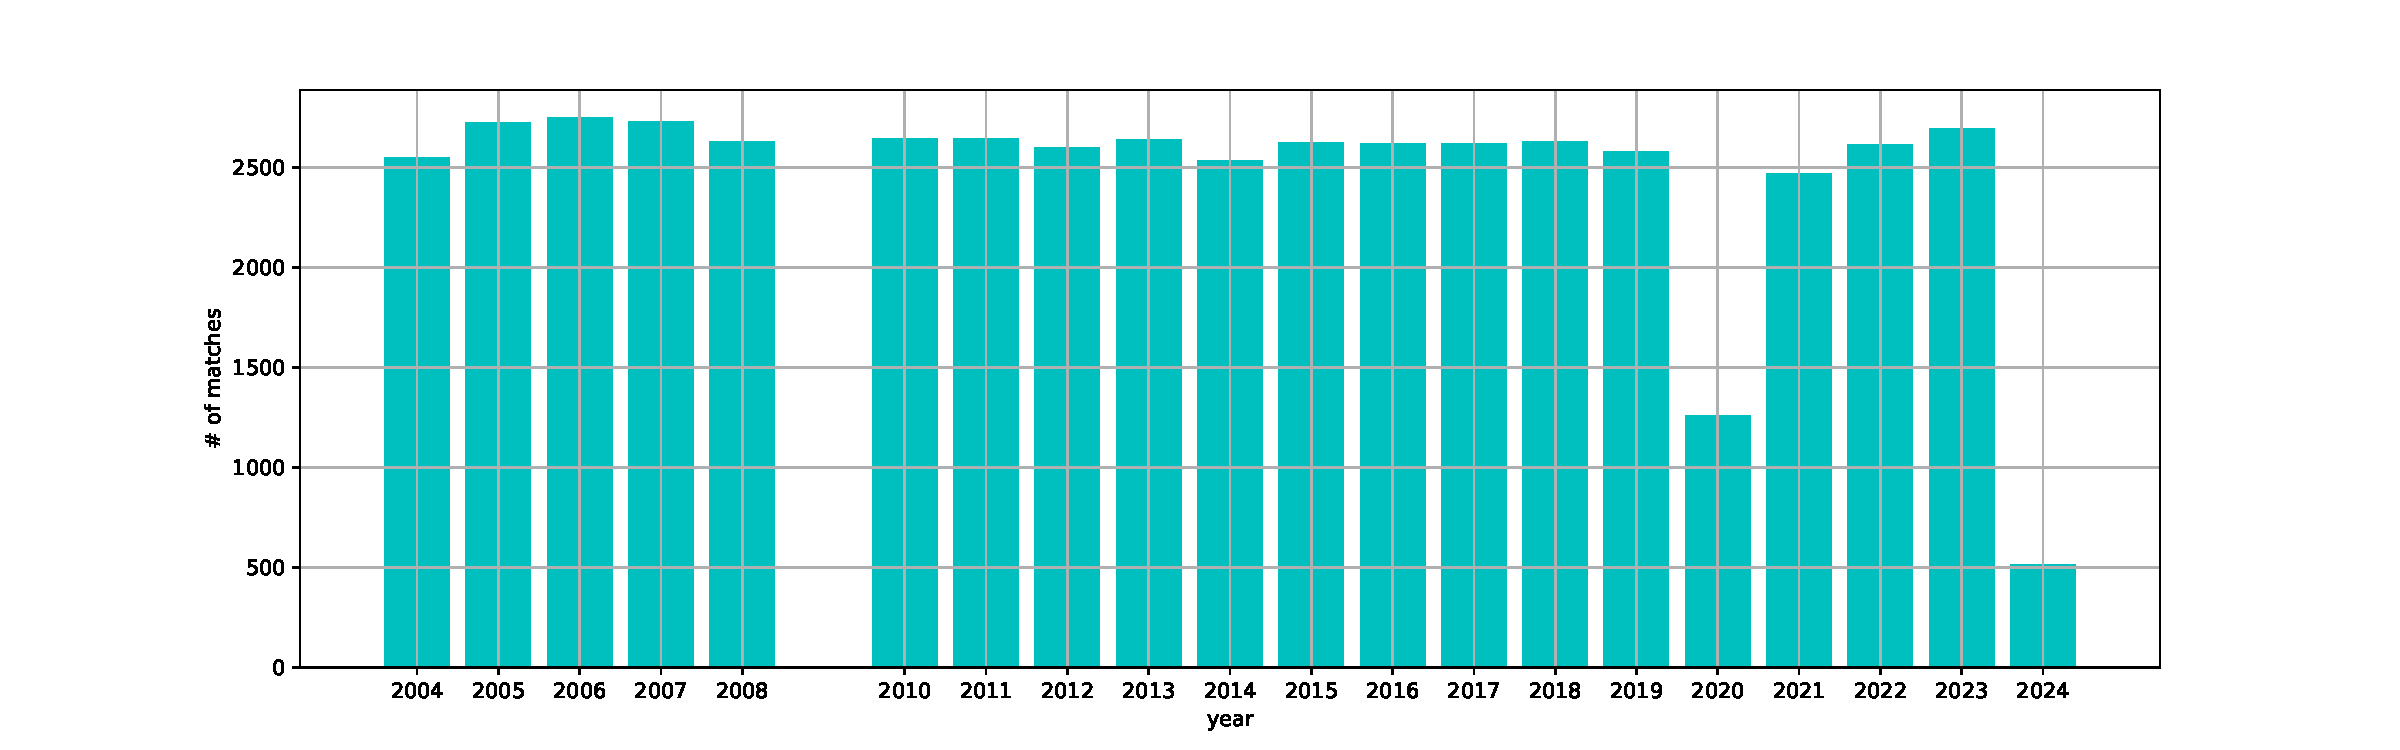
\includegraphics[width=\textwidth]{pictures/match-count-year-dist.pdf}
\caption{Count of Matches for each year in our dataset. Data has been obtained from \href{http://tennis-data.co.uk/}{tennis-data}.}
\label{match-count-year-dist}
\end{figure}
%
One of the most important metrics for assessing the performance of individual players in tennis is the Elo rating. The distribution of Elo ratings on the ATP tours reveals that the median rating is $1640$ (Figure \ref{elo-rates-dist}). Interestingly, only one player (N. Djokovic) has an Elo rate exceeding $2000$ (Figure \ref{top-25-elo-rates}).
%
\begin{figure}[h]
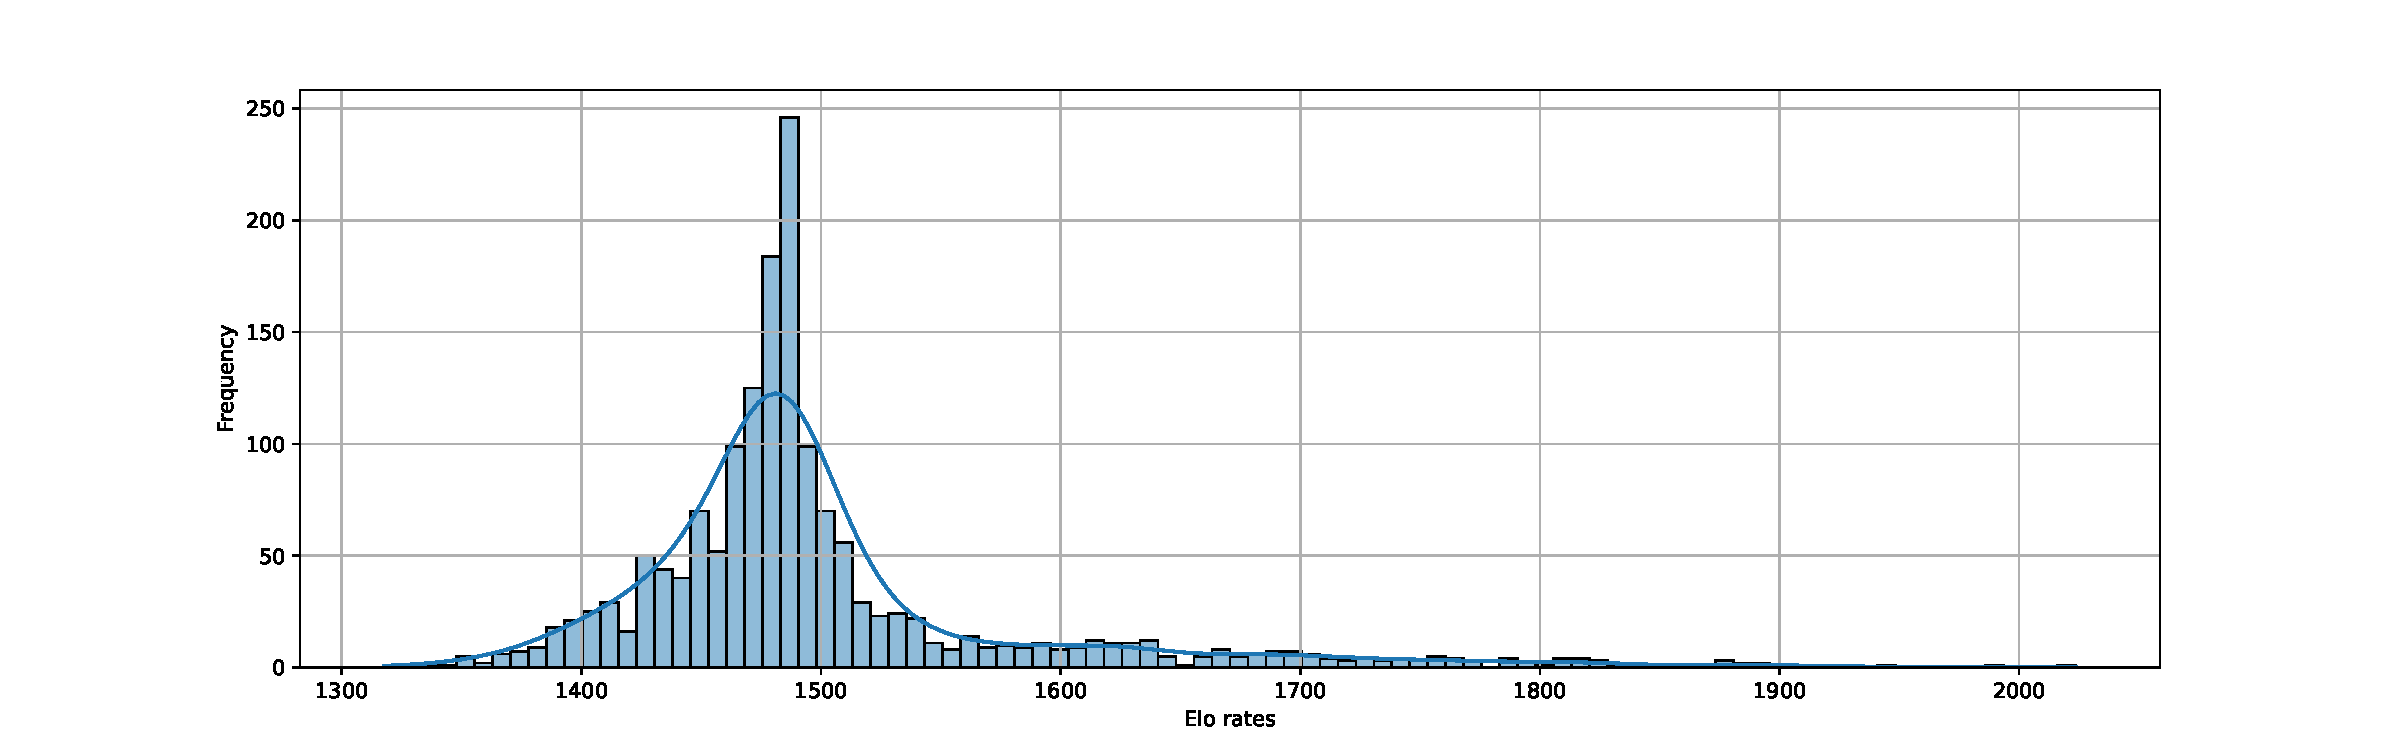
\includegraphics[width=\textwidth]{pictures/elo-rates-dist.pdf}
\caption{Distribution of Elo rates}
\label{elo-rates-dist}
\end{figure}
%
%
\begin{figure}[h]
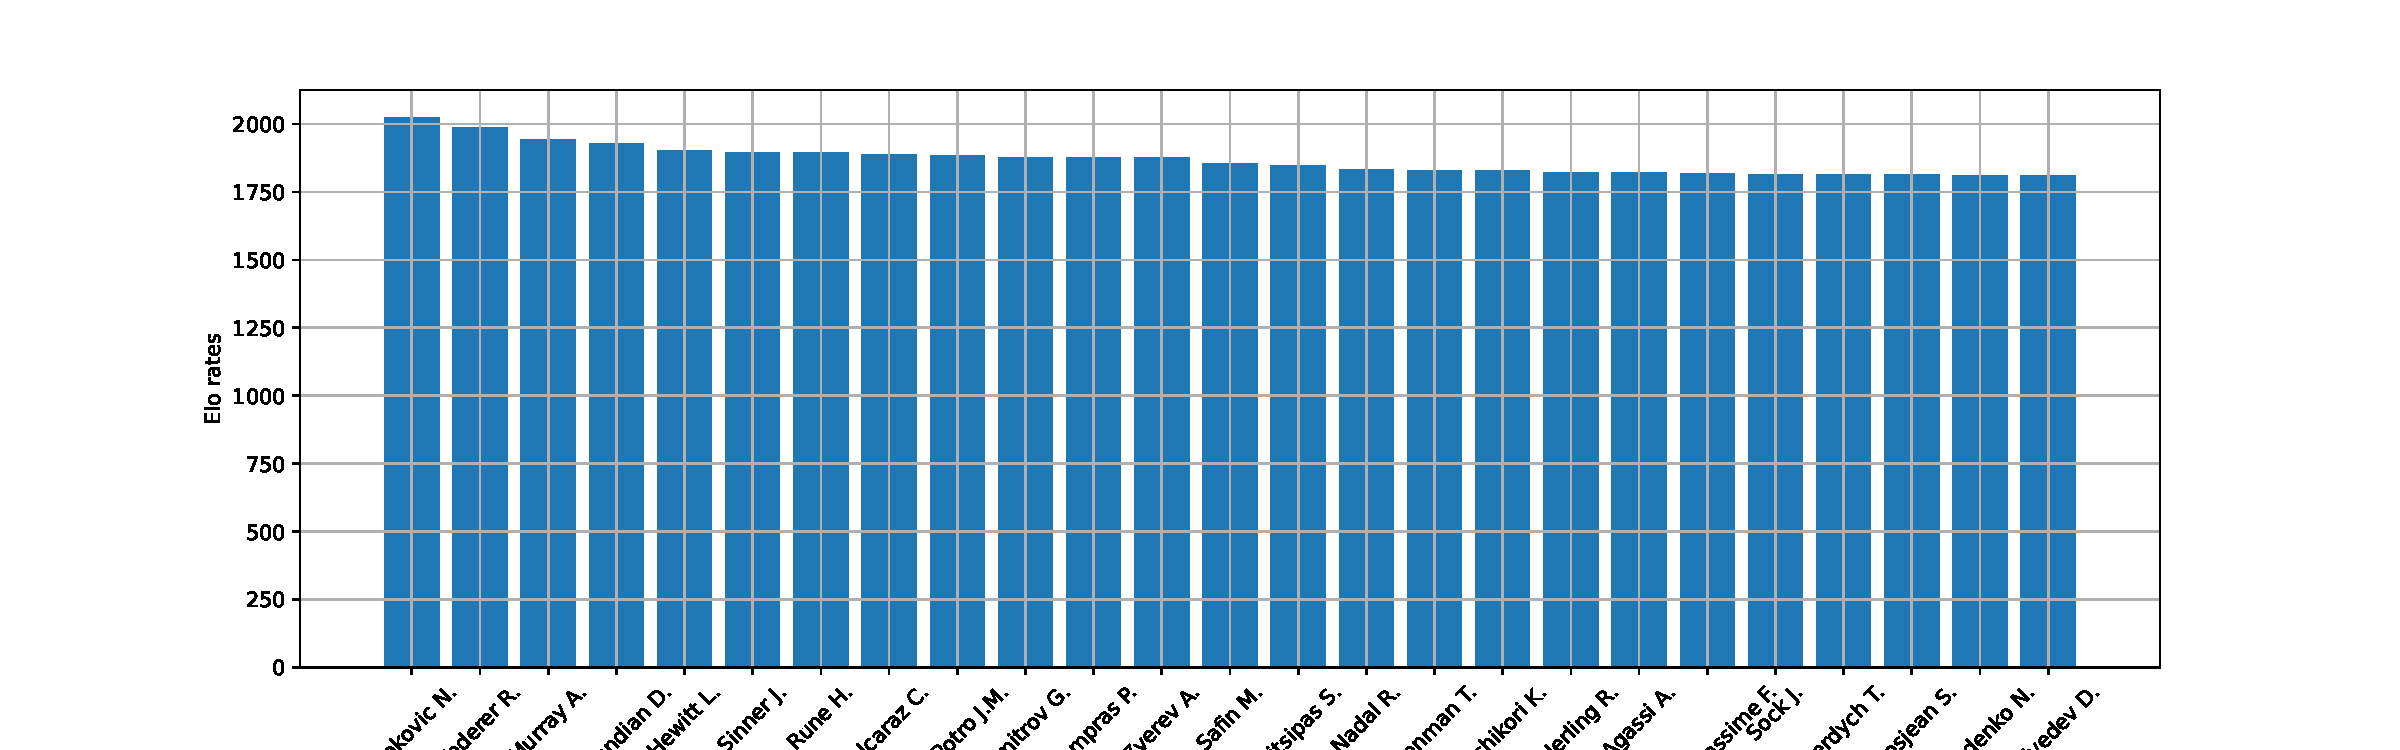
\includegraphics[width=\textwidth]{pictures/top-25-elo-rates.pdf}
\caption{Top 25 players with highest Elo rates: With an Elo rate above $1700$, a player would be among the top five percent of all players on the ATP tour.}
\label{top-25-elo-rates}
\end{figure}
%
Each player on the ATP tour starts with an Elo rating of $1500$ points. In our dataset, E. Prodon has the lowest Elo rating, with the rate of $1366$ (Figure \ref{bottom-25-elo-rates}).
%
\begin{figure}[h]
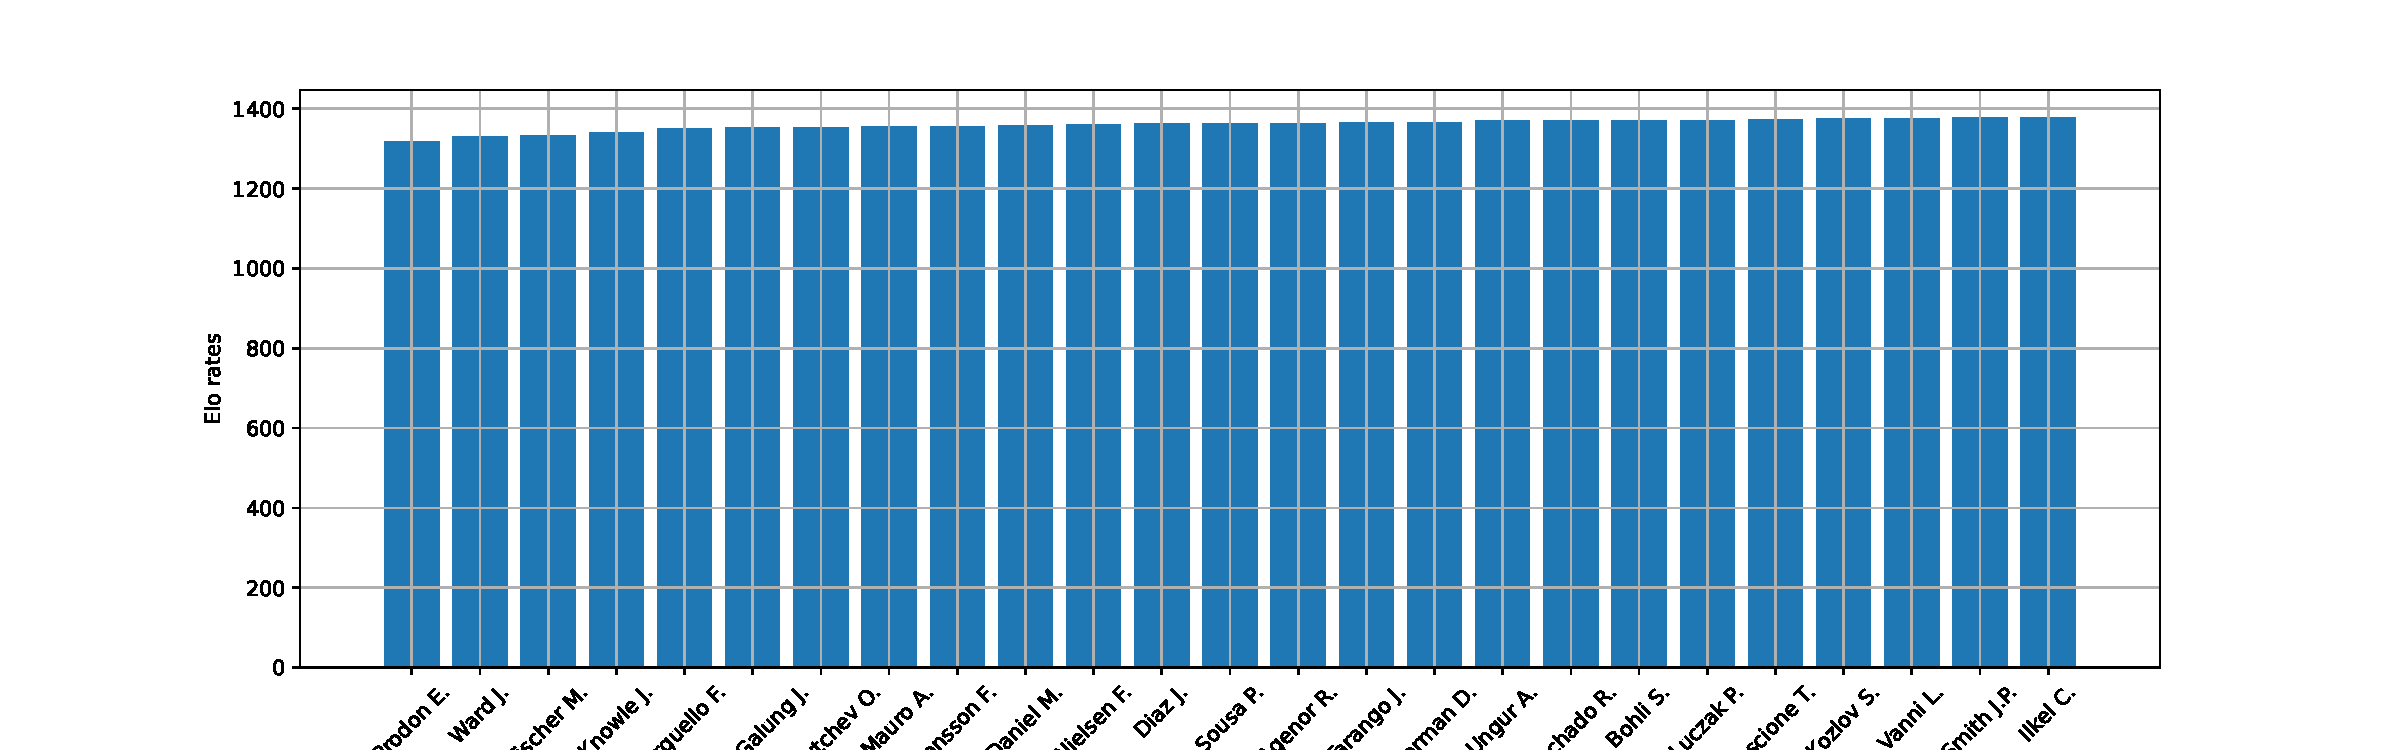
\includegraphics[width=\textwidth]{pictures/bottom-25-elo-rates.pdf}
\caption{Bottom 25 players with lowest Elo rates}
\label{bottom-25-elo-rates}
\end{figure}
%

To analyze if Elo rates differ for each player based on their performance on different court surfaces, we calculated ``surface-specific Elo rates'' (Figure \ref{top-10-elo-rates-indoor-carpet}, \ref{top-10-elo-rates-indoor-clay}, \ref{top-10-elo-rates-indoor-hard}, \ref{top-10-elo-rates-outdoor-clay}, \ref{top-10-elo-rates-outdoor-grass}, \ref{top-10-elo-rates-outdoor-hard}). Although players with higher Elo rates generally have higher surface-specific Elo ratings, certain players perform slightly better or worse based on the surface of the tennis court. This could be a critical factor for a machine learning model to classify which player wins if two players with almost identical Elo ratings play against each other.
%
\begin{figure}[h]
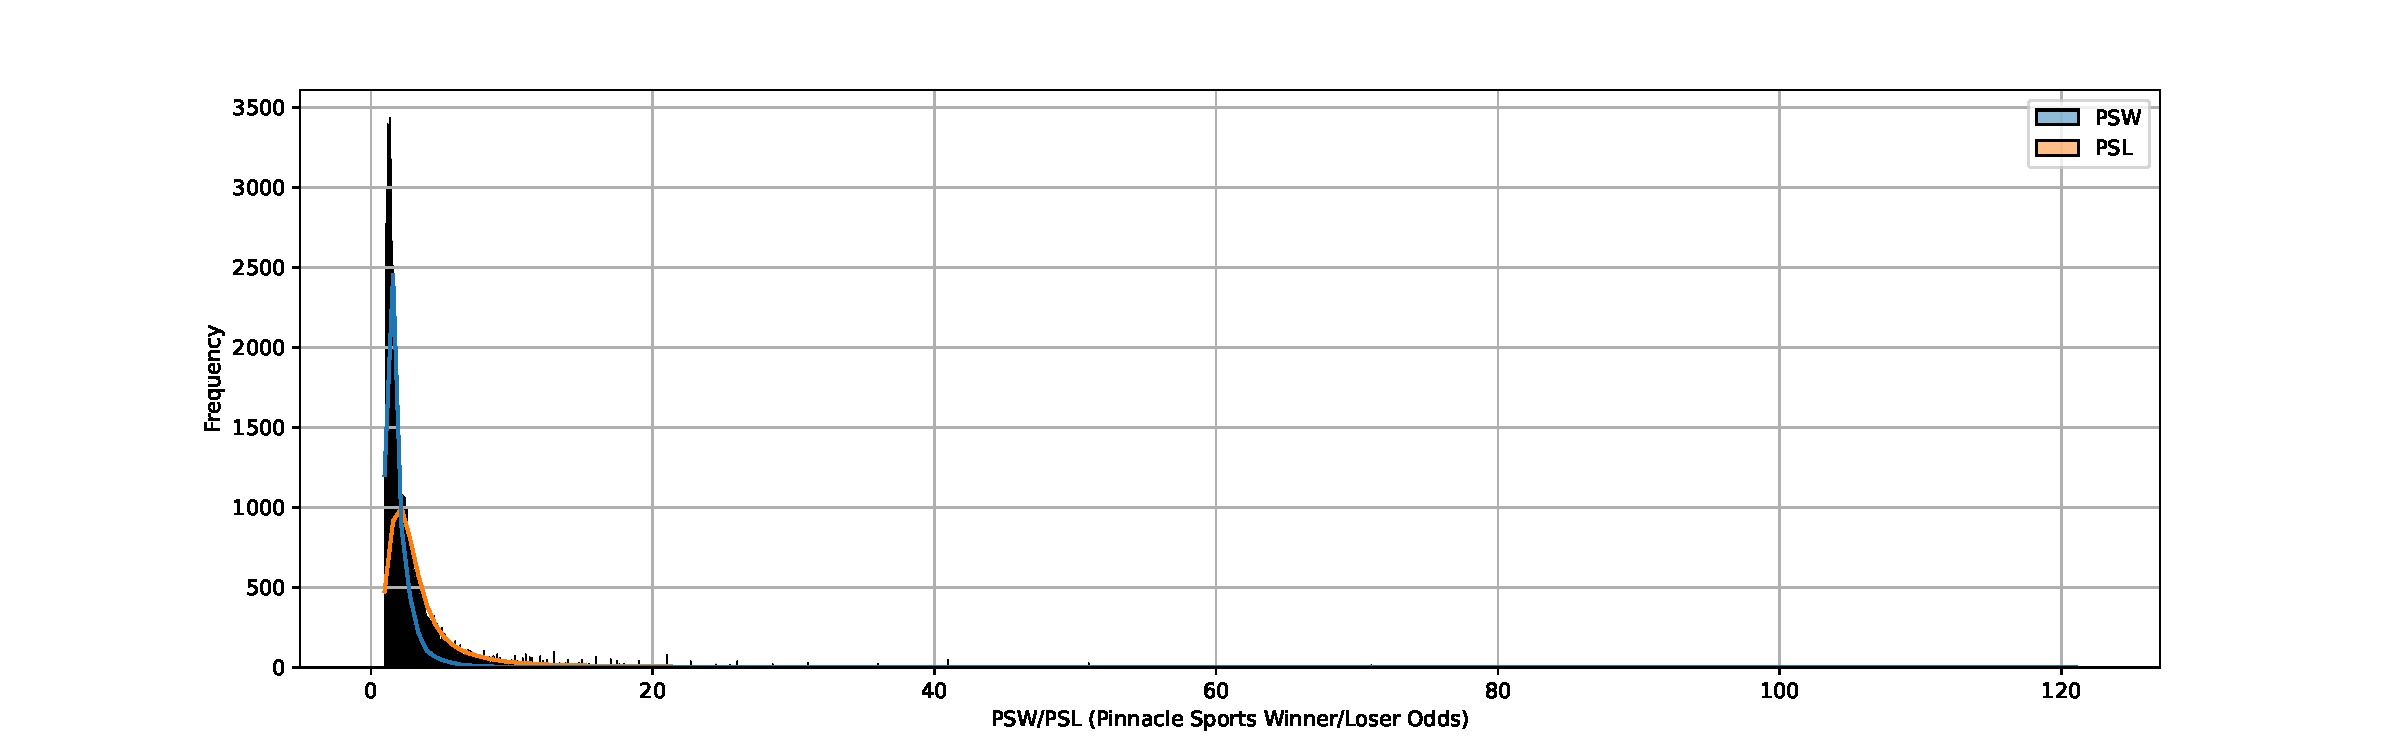
\includegraphics[width=\textwidth]{pictures/ps-odds-dist.pdf}
\caption{Distribution of Pinnacle Sports Winner/Loser Odds}
\label{ps-odds-dist}
\end{figure}
%
%
\begin{figure}[h]
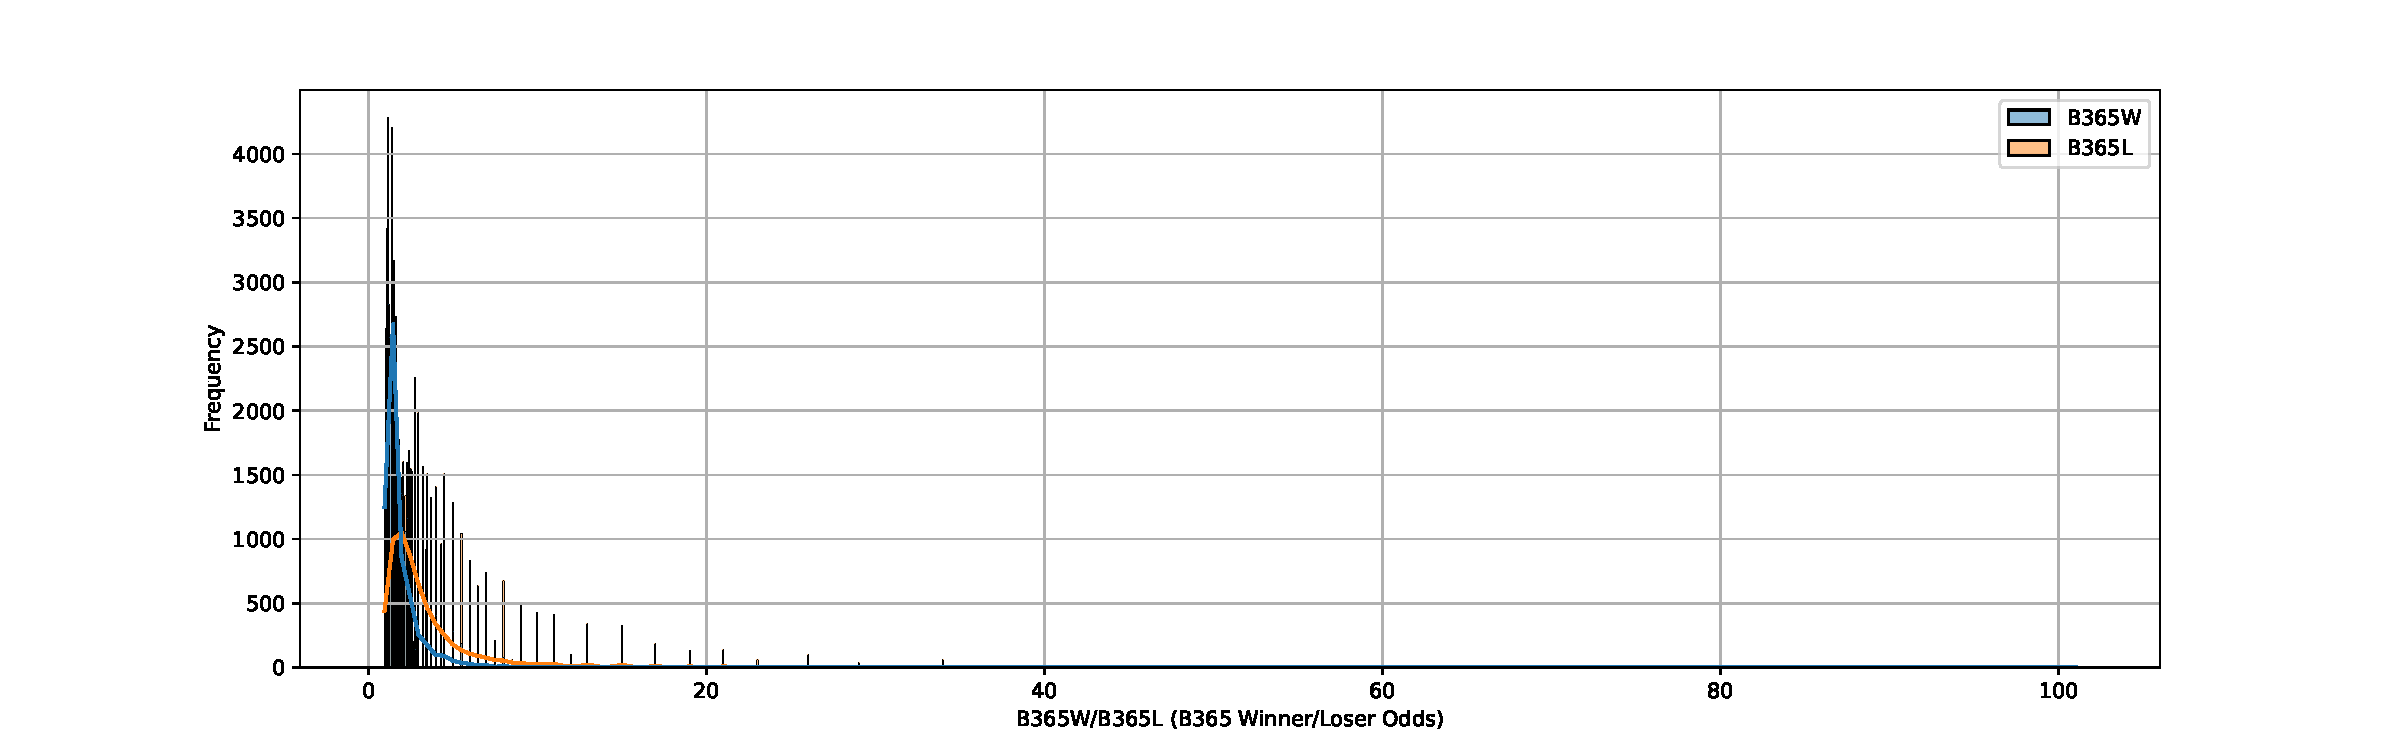
\includegraphics[width=\textwidth]{pictures/b365-odds-dist.pdf}
\caption{Distribution of B365 Winner/Loser Odds}
\label{b365-odds-dist}
\end{figure}
%
%
\begin{figure}[h]
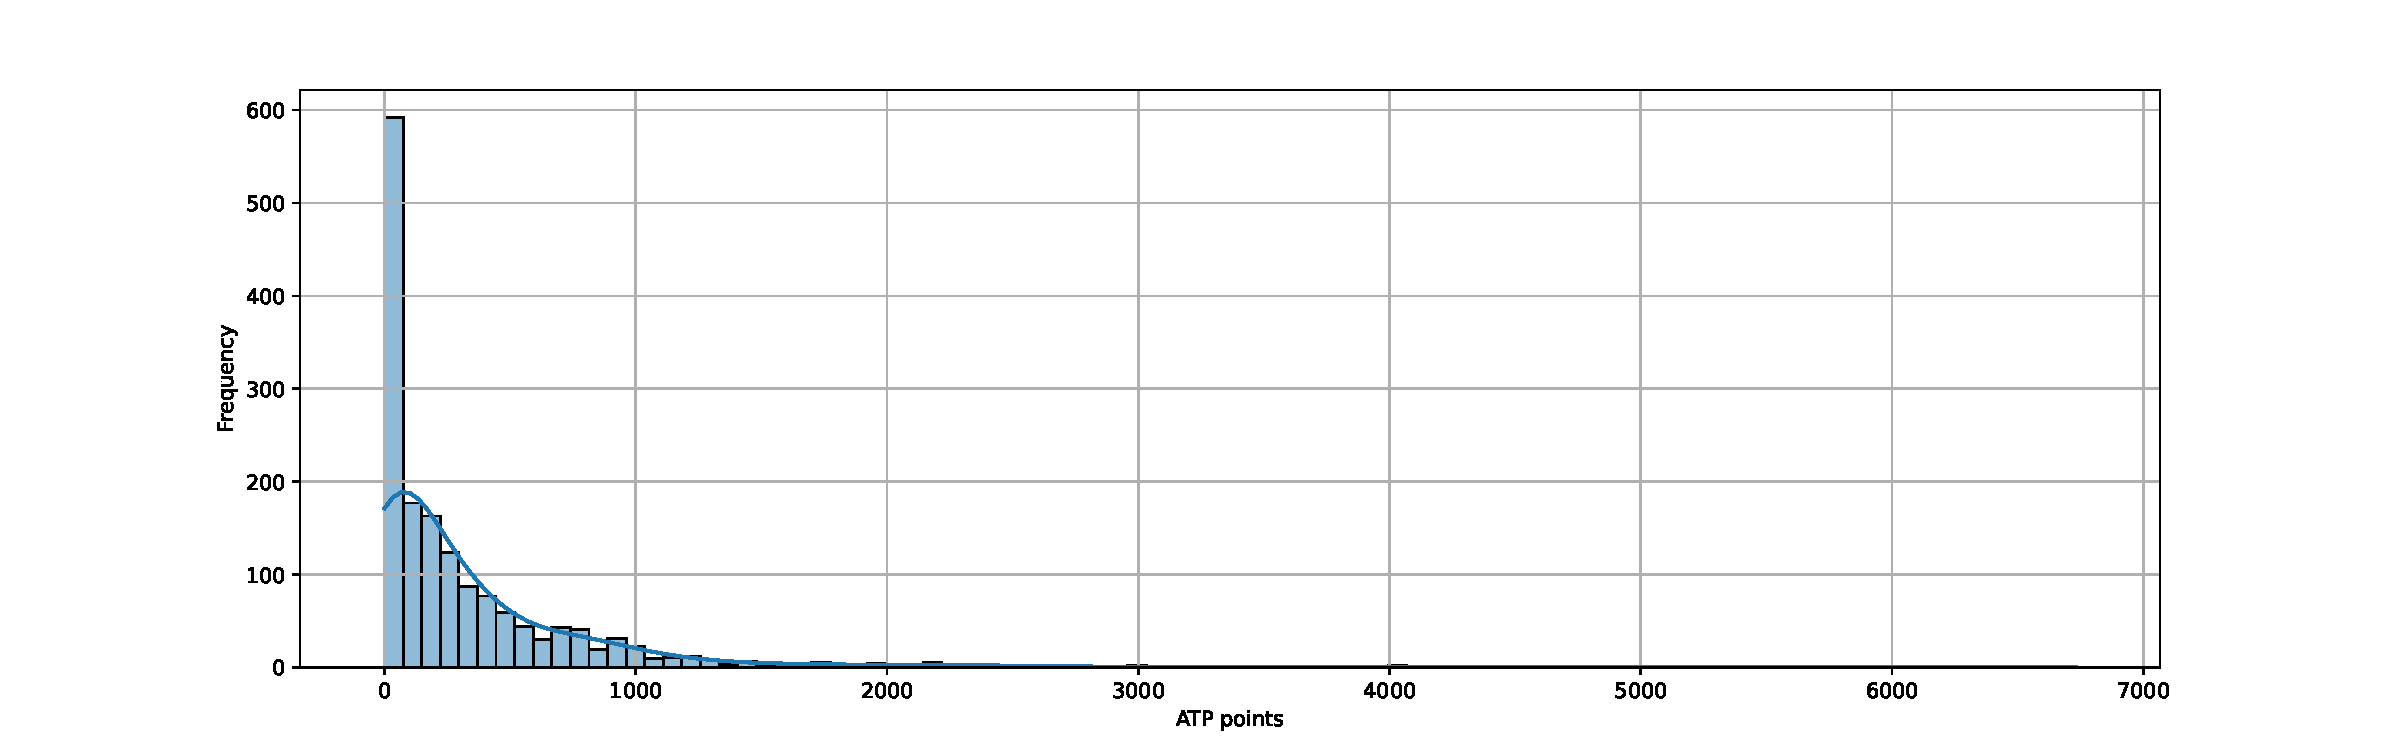
\includegraphics[width=\textwidth]{pictures/atp-point-dist.pdf}
\caption{Distribution of atp points}
\label{atp-point-dist}
\end{figure}
%
%
\begin{figure}[h]
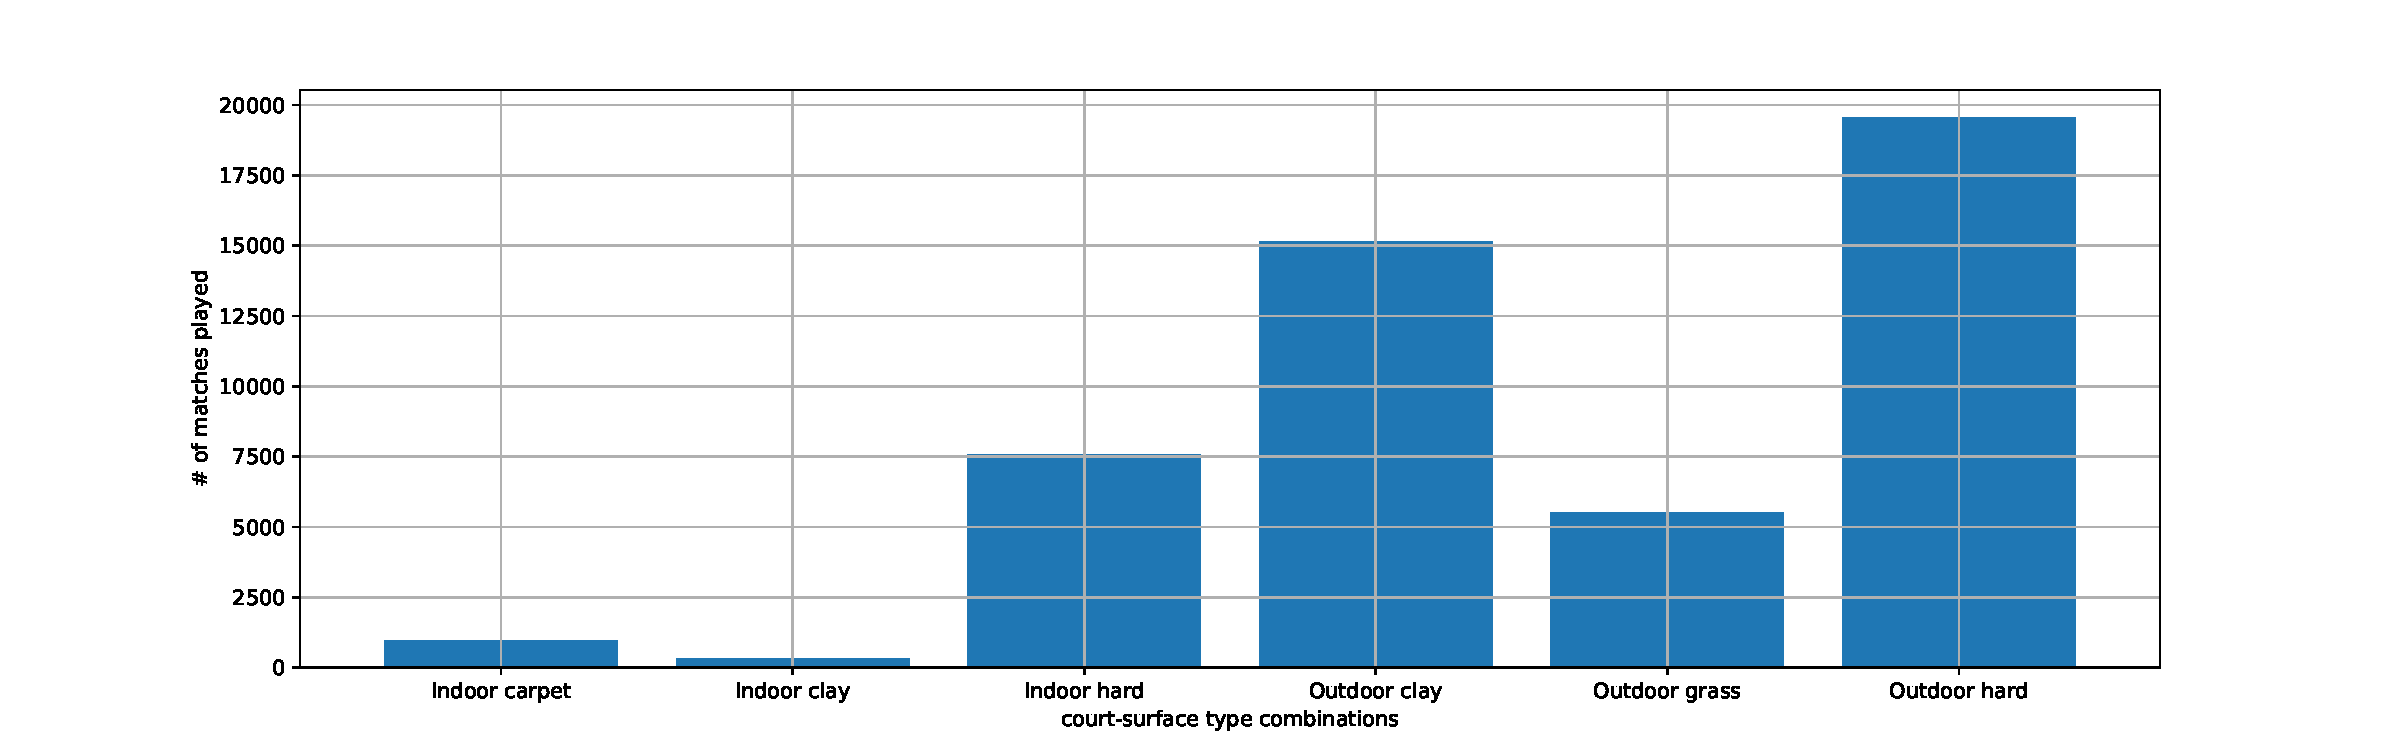
\includegraphics[width=\textwidth]{pictures/match-count-field-type-dist.pdf}
\caption{Total number of matches held on each court/surface type}
\label{match-count-field-type-dist}
\end{figure}
%
%
\begin{figure}[h]
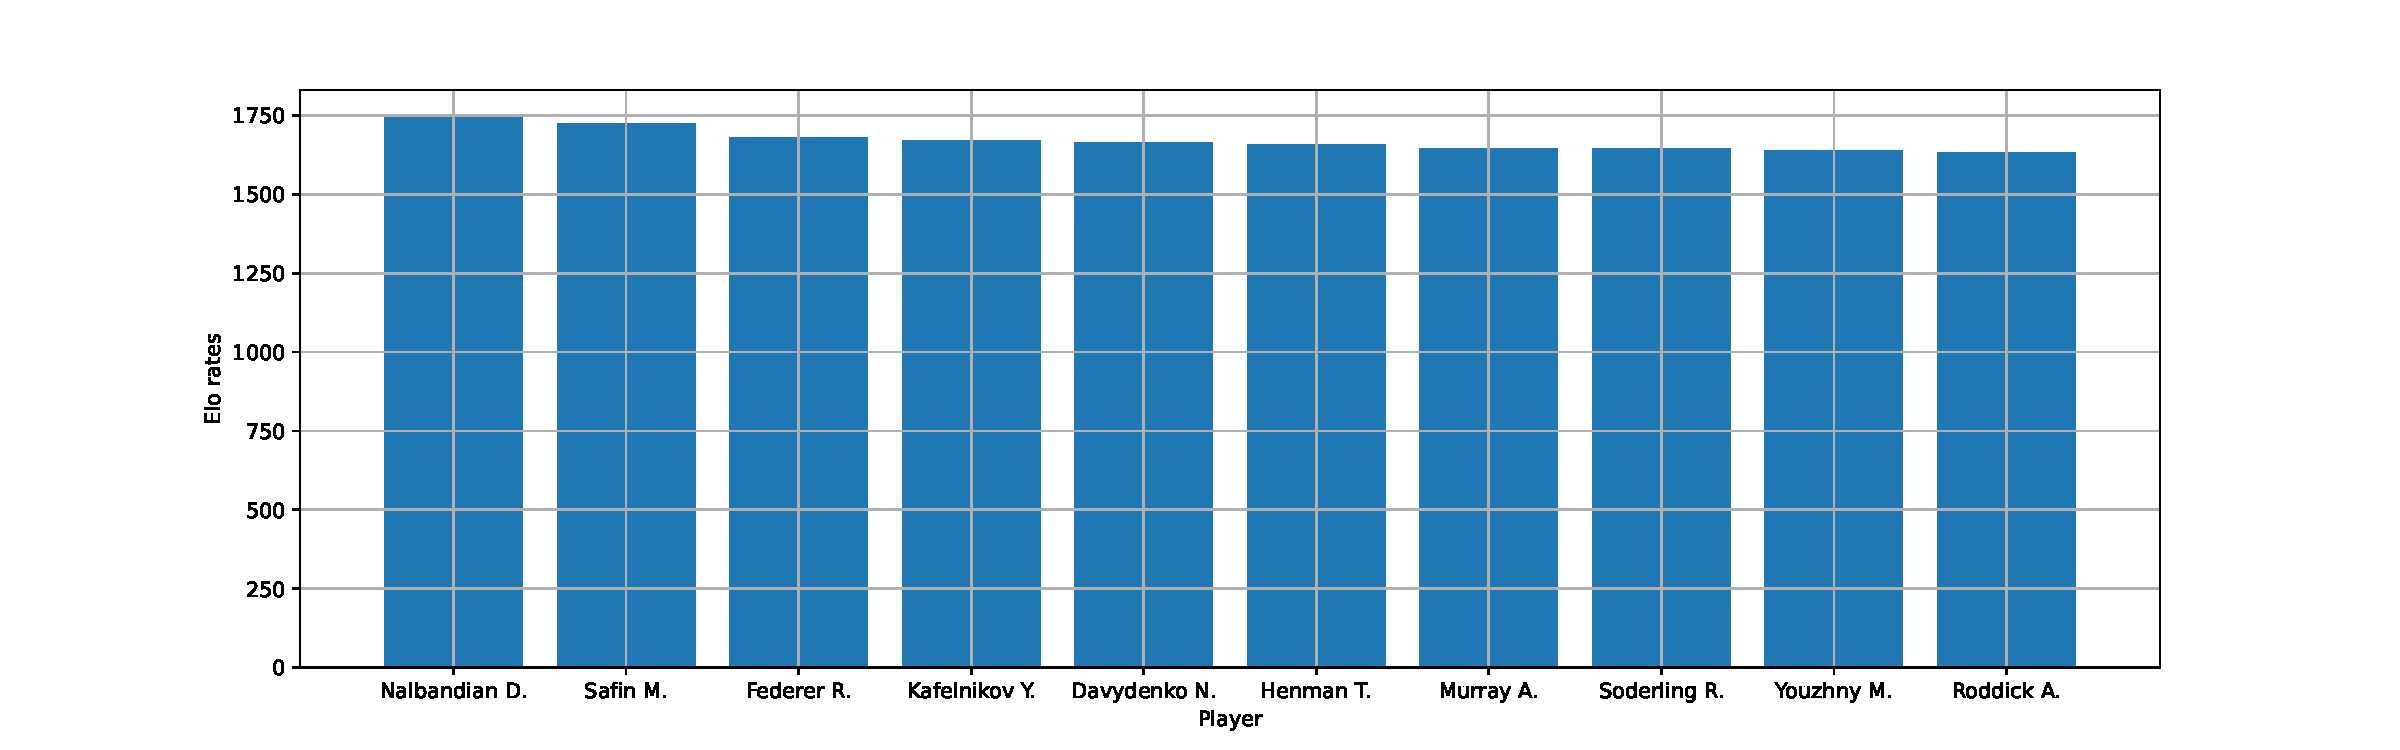
\includegraphics[width=\textwidth]{pictures/top-10-elo-rates-indoor-carpet.pdf}
\caption{Top 10 players in indoor courts and on carpet surfaces}
\label{top-10-elo-rates-indoor-carpet}
\end{figure}
%
%
\begin{figure}[h]
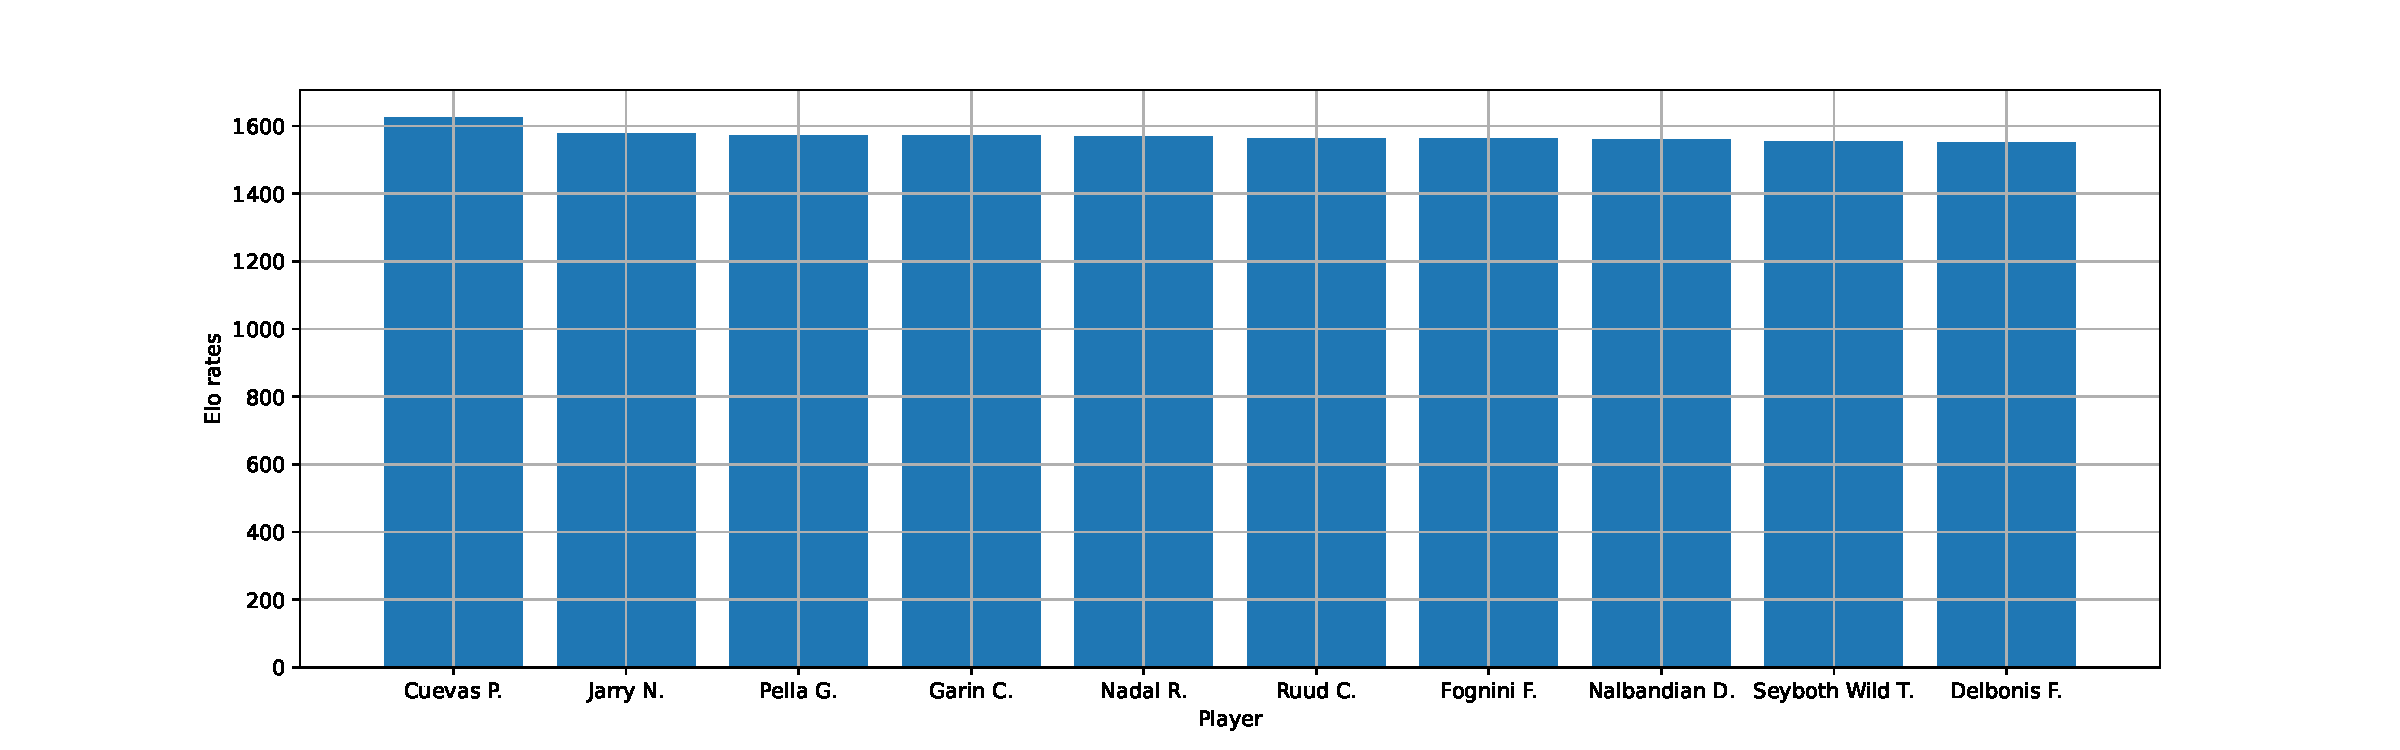
\includegraphics[width=\textwidth]{pictures/top-10-elo-rates-indoor-clay.pdf}
\caption{Top 10 players in indoor courts and on clay surfaces}
\label{top-10-elo-rates-indoor-clay}
\end{figure}
%
%
\begin{figure}[h]
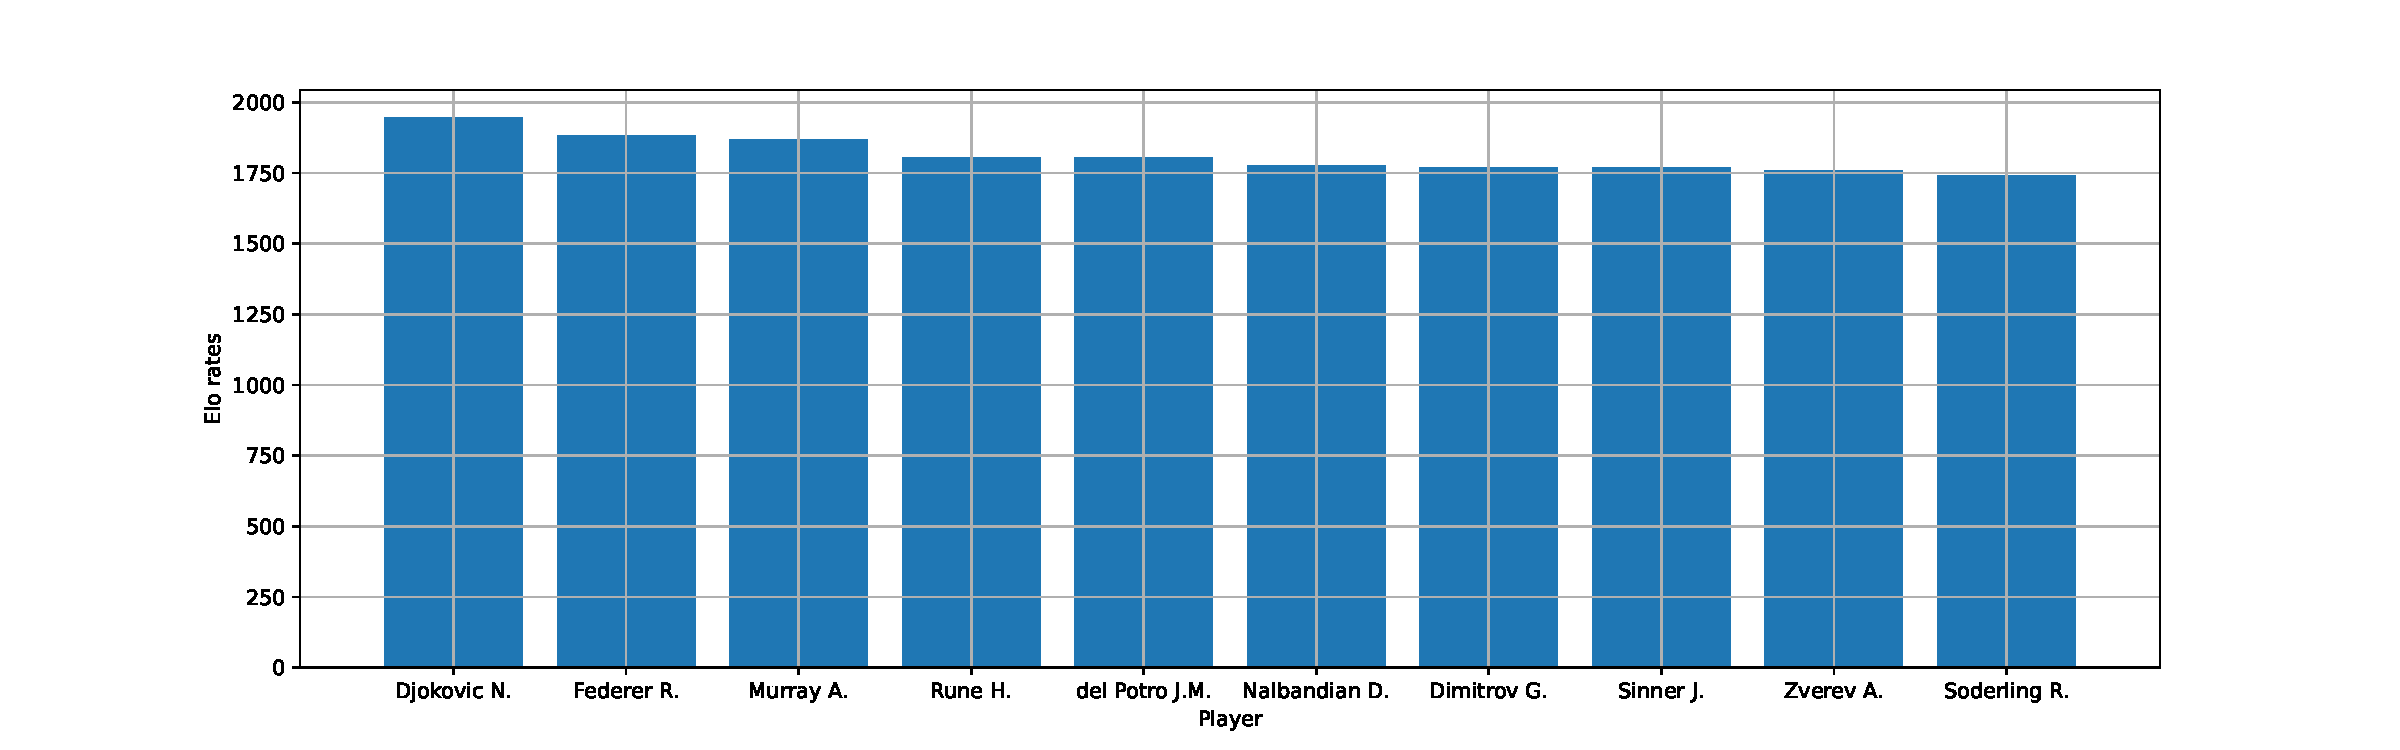
\includegraphics[width=\textwidth]{pictures/top-10-elo-rates-indoor-hard.pdf}
\caption{Top 10 players in indoor courts and on hard surfaces}
\label{top-10-elo-rates-indoor-hard}
\end{figure}
%
%
\begin{figure}[h]
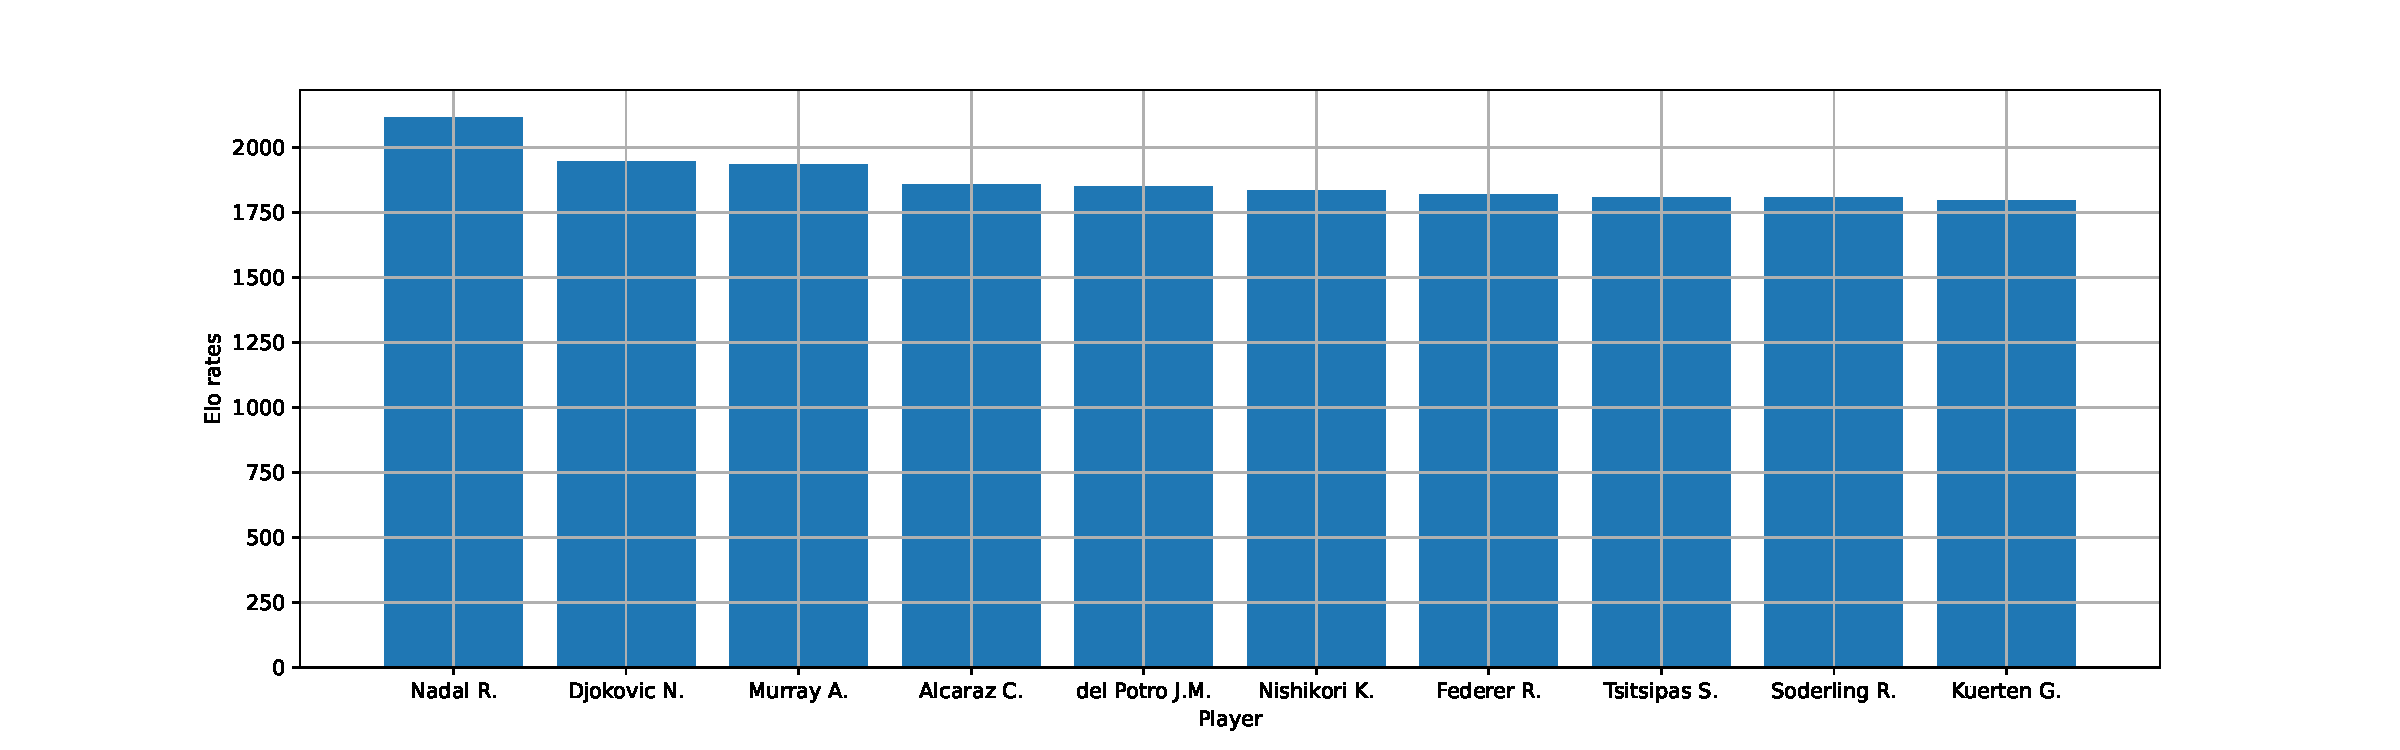
\includegraphics[width=\textwidth]{pictures/top-10-elo-rates-outdoor-clay.pdf}
\caption{Top 10 players in outdoor courts and on clay surfaces}
\label{top-10-elo-rates-outdoor-clay}
\end{figure}
%
%
\begin{figure}[h]
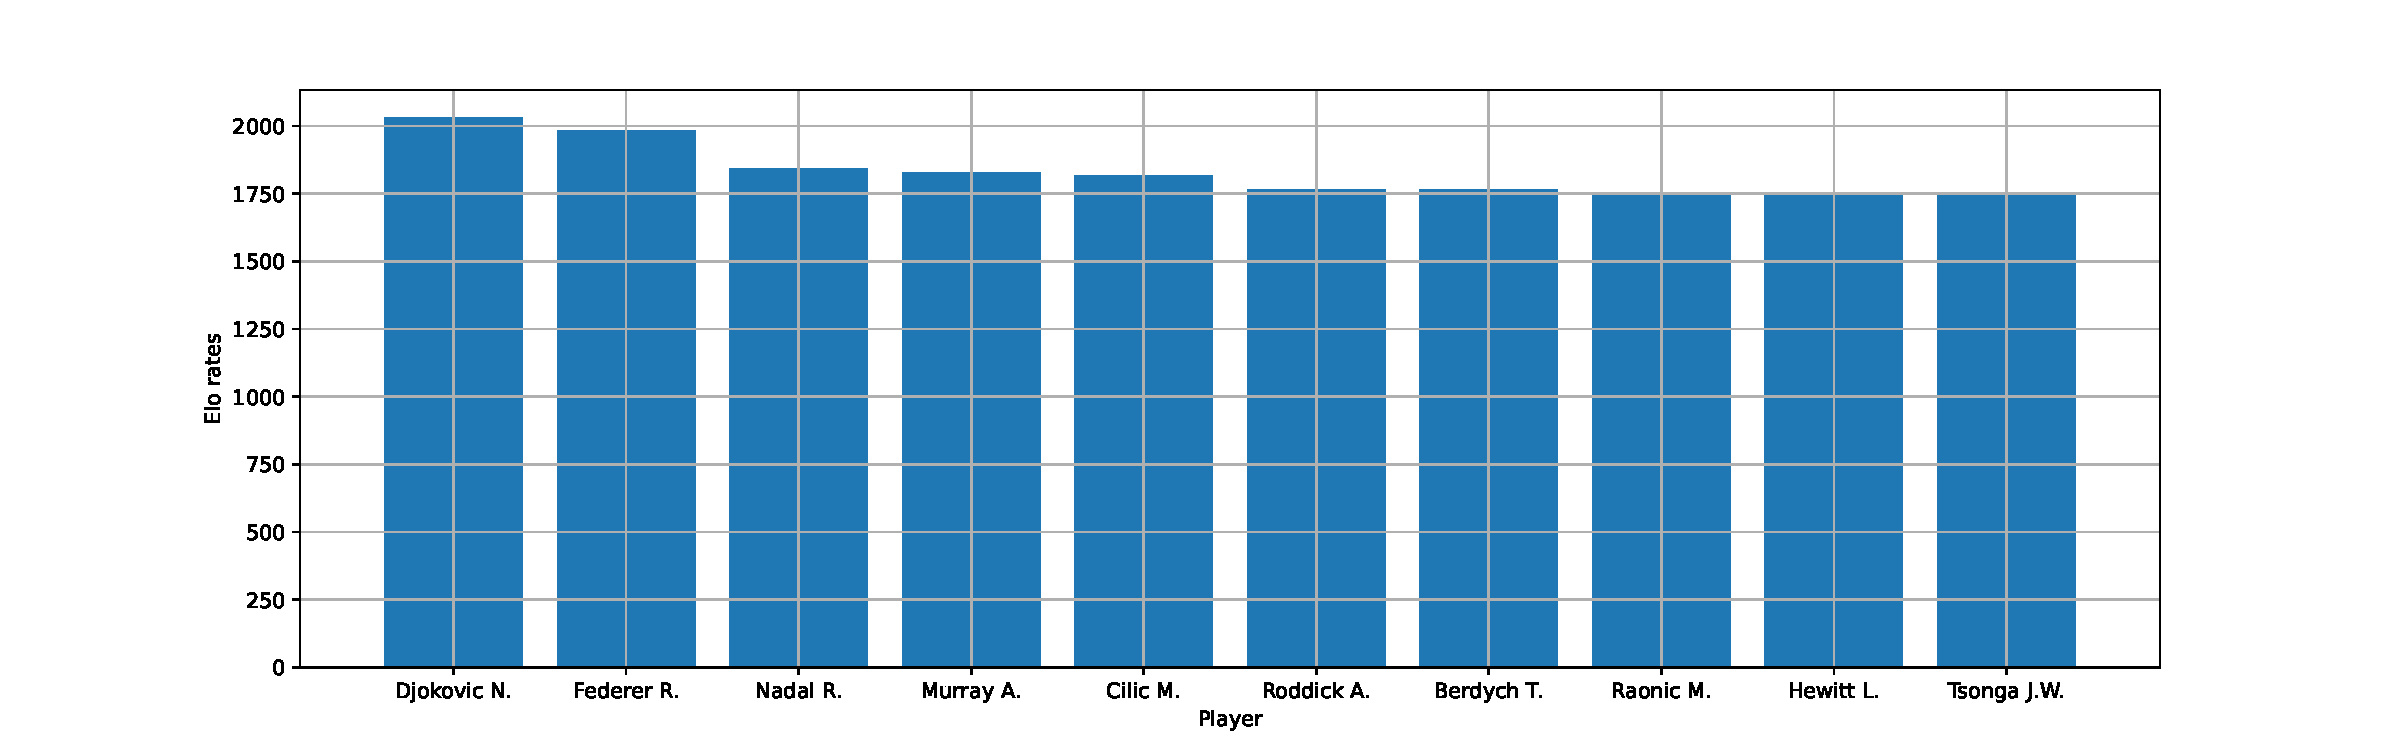
\includegraphics[width=\textwidth]{pictures/top-10-elo-rates-outdoor-grass.pdf}
\caption{Top 10 players in outdoor courts and on grass surfaces}
\label{top-10-elo-rates-outdoor-grass}
\end{figure}
%
%
\begin{figure}[h]
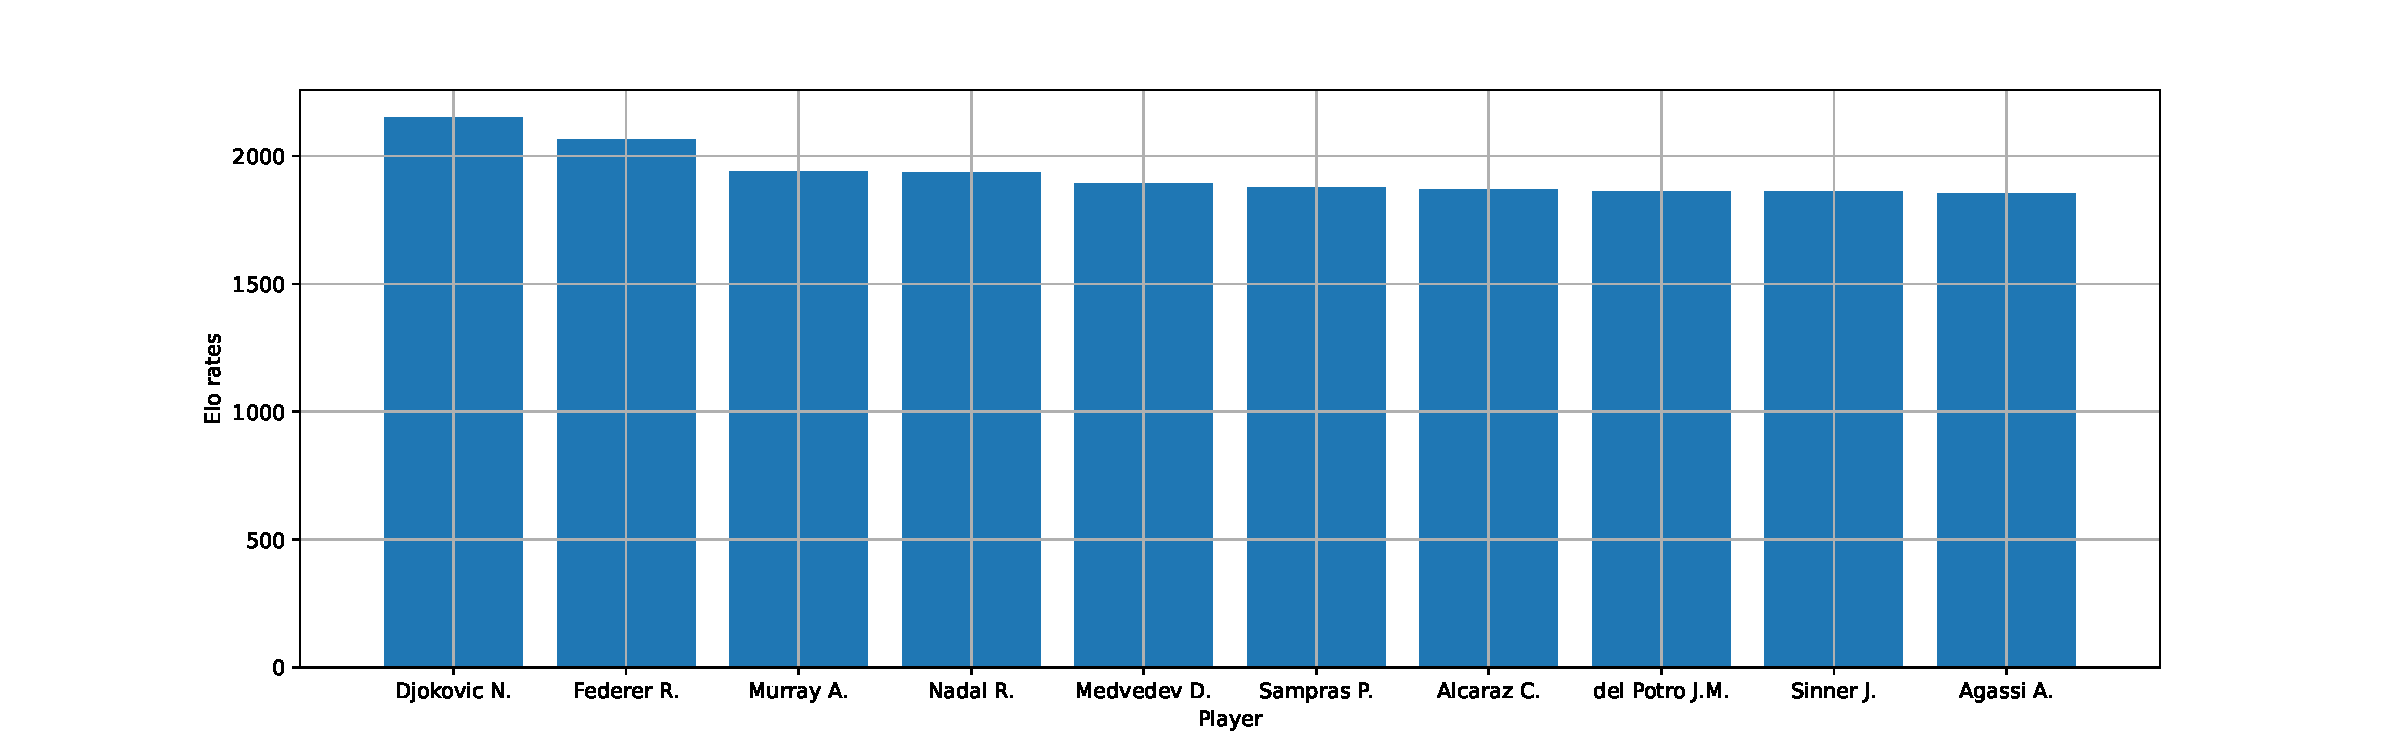
\includegraphics[width=\textwidth]{pictures/top-10-elo-rates-outdoor-hard.pdf}
\caption{Top 10 players in outdoor courts and on hard surfaces}
\label{top-10-elo-rates-outdoor-hard}
\end{figure}
%

A comparison of the players with the top 40 match wins shows that Djokovic, Nadal, and Federer were the most successful tennis players in recent history (Figure \ref{top-40-players-match-wins}), each with over 800 match wins. This observation is further supported by the average Elo ratings as well as the surface-specific Elo ratings. Not surprisingly, the players with the most match wins also have the most tournament wins (Figure \ref{top-40-players-tournament-wins}).
%
\begin{figure}[h]
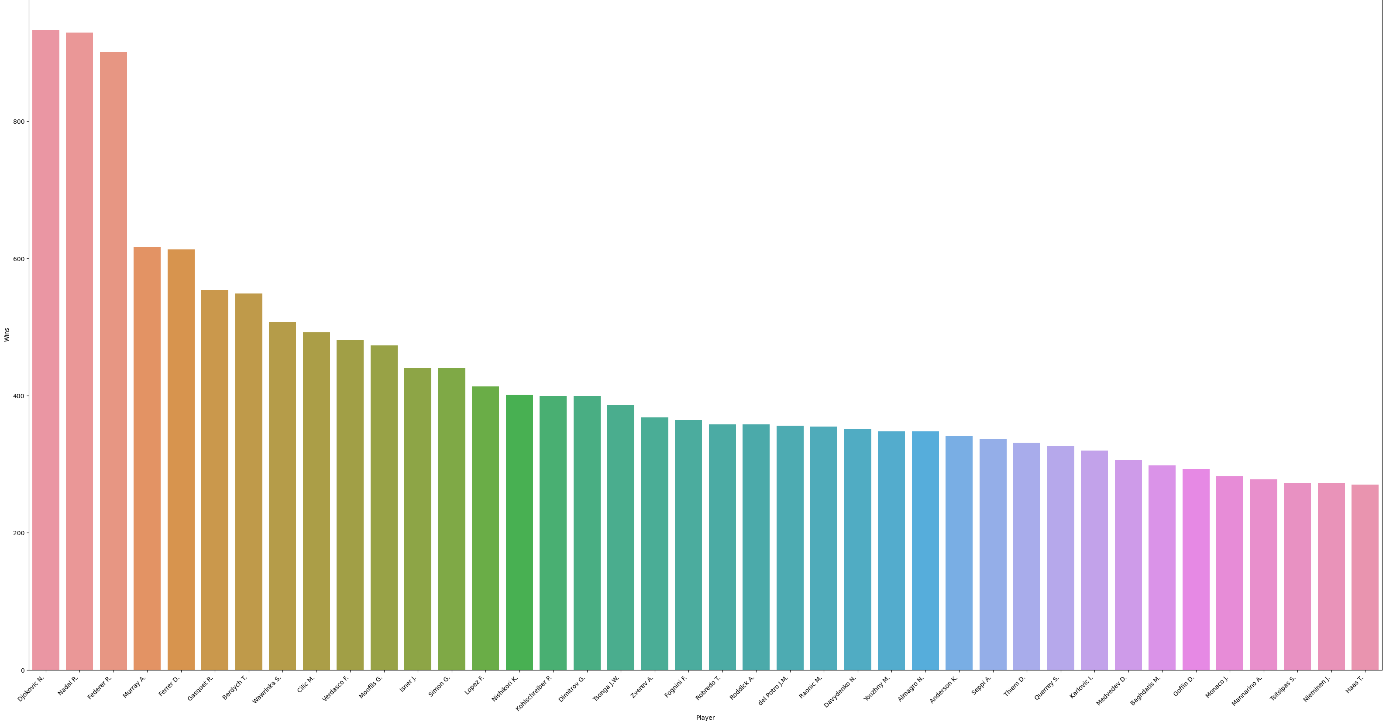
\includegraphics[width=\textwidth]{pictures/top-40-players-match-wins.png}
\caption{Top 40 players based on the total match wins}
\label{top-40-players-match-wins}
\end{figure}
%
%
\begin{figure}[h]
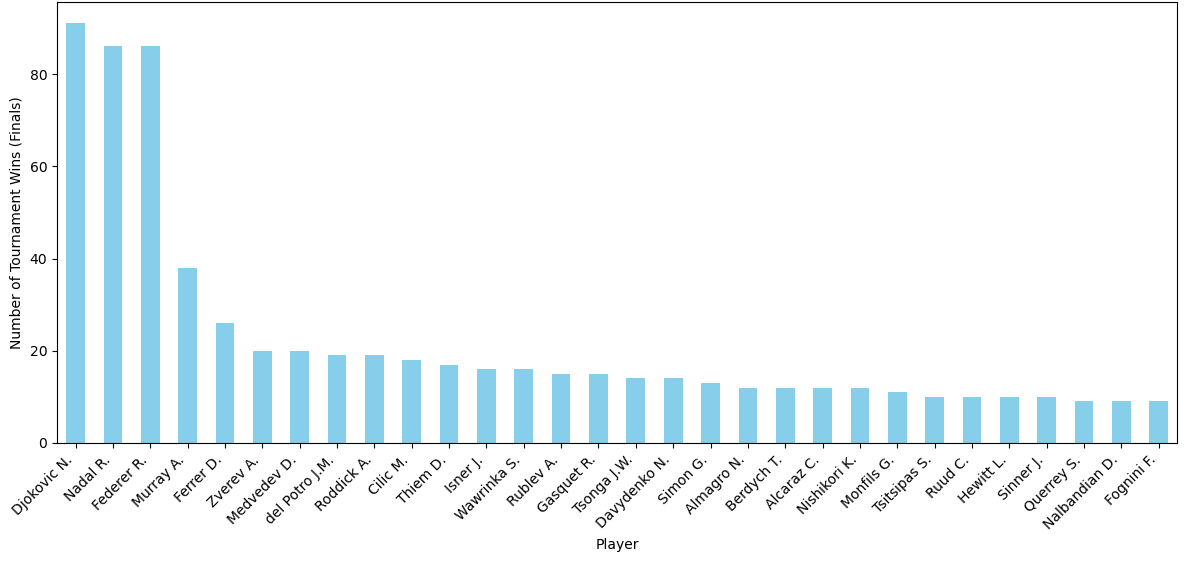
\includegraphics[width=\textwidth]{pictures/top-40-players-tournament-wins.png}
\caption{Top 40 players based on the total tournament wins}
\label{top-40-players-tournament-wins}
\end{figure}
%

As it is observed, Elo rates are highly concentrated about 1500 in indoor carpet and clay field types in comparison with other court/surface types. This means that Elo rates in these field types carry less information about the skills of the players, as they have more or less the same rates (Figure \ref{elo-rate-field-type-dist}). Accordingly and also considering the low number of matches played on those court/suface types (Figure \ref{match-count-field-type-dist}), it does not sound reasonable to rely on the Elo rate for outcome forecasting in those field types.
%
\begin{figure}[h]
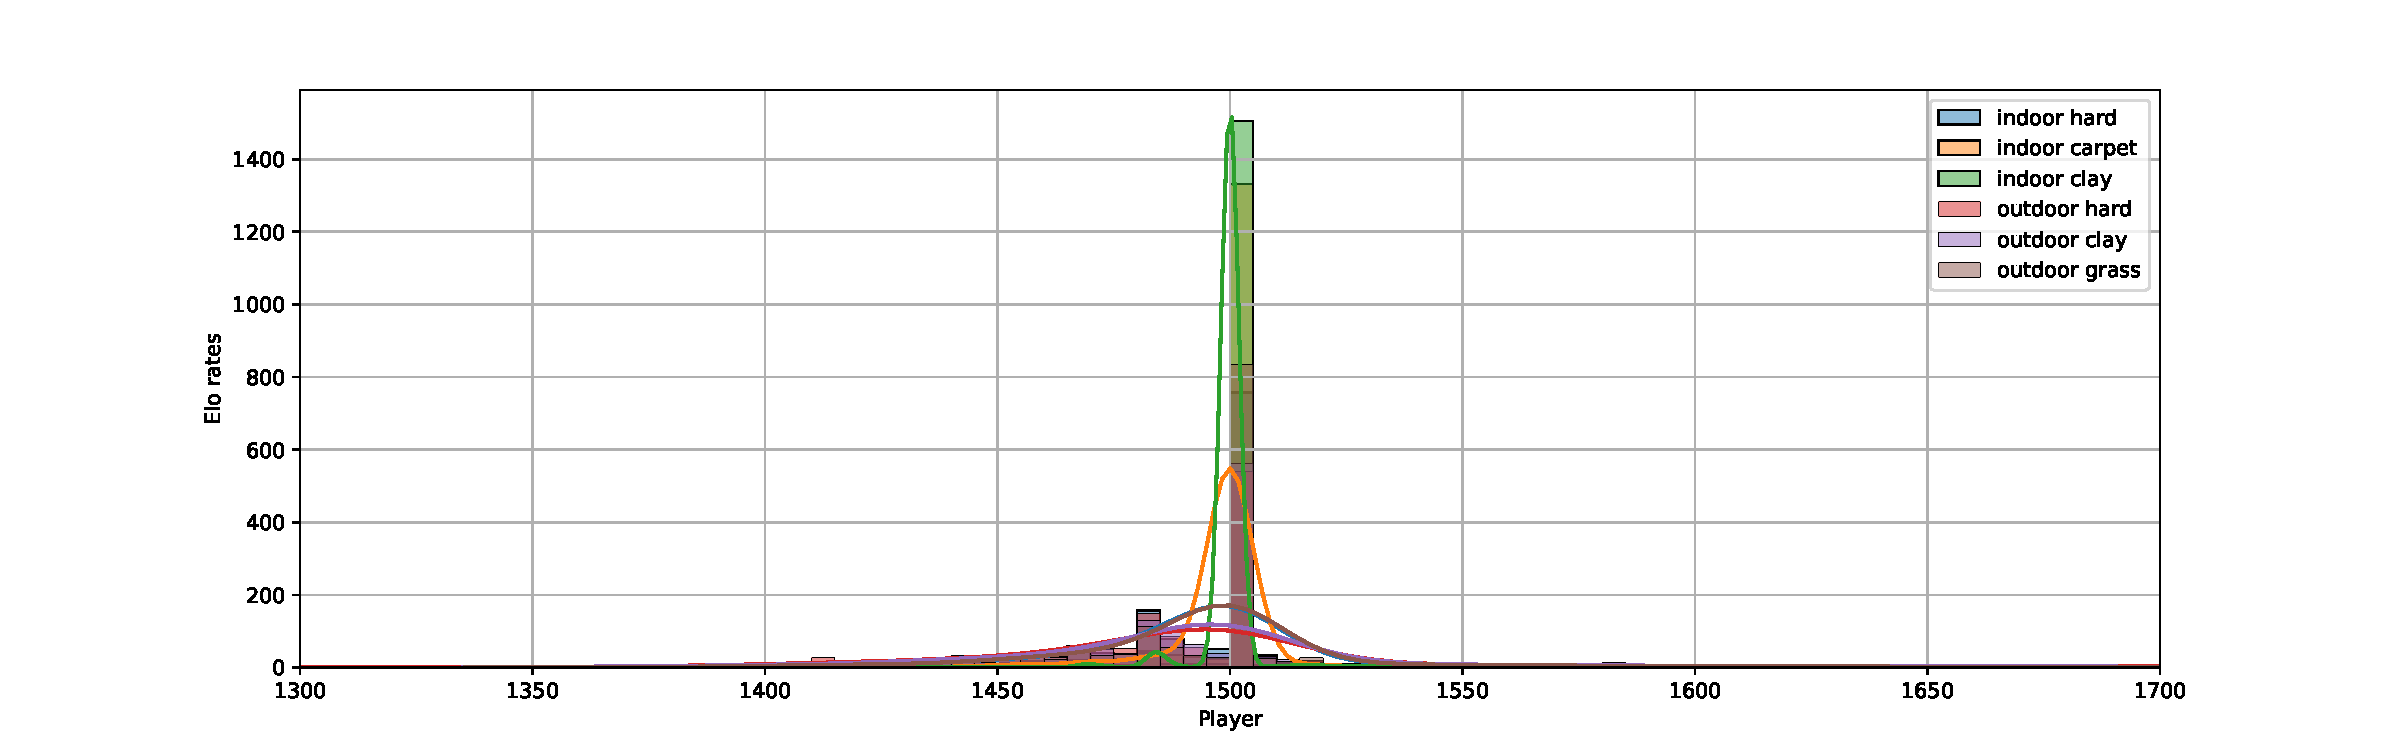
\includegraphics[width=\textwidth]{pictures/elo-rate-field-type-dist.pdf}
\caption{This graph shows the distribution of Elo rates on all court/surface type combinations.}
\label{elo-rate-field-type-dist}
\end{figure}
%


\subsection{Strategies}

To show how the some of the main features we used in the dataset how our ML models will add predictablity power, we defined a few betting strategies solely based on the parameters defined previously. Further, we defined some other theoretical bet strategies such as always winner/loser and random bet strategy, that are not real bet strategy, but are the test cases (base line) for the future analysis instead. These bet strategies were defined as follows:
%
\begin{enumerate}
\item To bet on the higher ranked player based on the atp point of either parties in each match (HPBS)
\item To bet on the lower ranked player based on the atp point of either parties in each match (LPBS)
\item To bet on the player with higher total elo rate in each match (HRBS)
\item To bet on the player with lower total elo rate in each match (LRBS)
\item To bet on the player with the better elo rate in the appropirate field type in each match (BRFTBS)
\item To bet on a random player (RPBS)
\item To bet on the winner in each match (WBS)
\item To bet on the loser in each match (LBS)
\end{enumerate}
%
Of course, strategies 7 and 8 are just theoretical and put there to be compared with other strategies and models as the maximum average profit/loss. Also, the random strategy is a good baseline to show if our model is forecasting any better than just blindly/randomly picking a player to bet. The first five strategy is showing how the main features of our models would perform financially and accurately on their own. Tables \ref{strategies-preformance-pinnacle-1}, \ref{strategies-preformance-pinnacle-2}, \ref{strategies-preformance-b365-1} and \ref{strategies-preformance-b365-2} show statistics of strategies' performances on ``Pinnacle'' and ``Bet 365'' platforms.
%
\begin{table}[h]
\centering
\caption{Strategies' performances on pinnacle part 1}
\begin{tabular}{|l|c|c|c|c|}
\hline
& \textbf{HPBS\_PS} & \textbf{LPBS\_PS} & \textbf{HRBS\_PS} & \textbf{LRBS\_PS} \\
\hline
mean & $-0.033897$ & $-0.048255$ & $-0.005117	$ & $-0.071235$ \\
\hline
std & $0.817451$ & $1.680054$ & $0.875762	$ & $1.651357$ \\
\hline
min & $-1.000000$ & $-1.000000$ & $-1.000000$ & $-1.000000$ \\
\hline
25\% & $-1.000000$ & $-1.000000$ & $-1.000000$ & $-1.000000$ \\
\hline
median & $0.180000$ & $-1.000000$ & $0.180000$ & $-1.000000$ \\
\hline
75\% & $0.476000$ & $0.794000$ & $0.500000$ & $0.700000$ \\
\hline
max & $11.000000$ & $45.000000$ & $14.000000$ & $45.000000$ \\
\hline
\end{tabular}

\label{strategies-preformance-pinnacle-1}
\end{table}
%
%
\begin{table}[h]
\centering
\caption{Strategies' performances on pinnacle part 2}
\begin{tabular}{|l|c|c|c|c|}
\hline
& \textbf{BRFTBS\_PS} & \textbf{RPBS\_PS} & \textbf{WBS\_PS} & \textbf{LBS\_PS} \\
\hline
mean & $0.006359$ & $-0.035683$ & $0.926425$ & $-1.000000$ \\
\hline
std & $0.929040$ & $1.323476$ & $1.281068$ & $0$ \\
\hline
min & $-1.000000$ & $-1.000000$ & $-0.028000$ & $-1.000000$ \\
\hline
25\% & $-1.000000$ & $-1.000000$ & $0.280000$ & $-1.000000$ \\
\hline
median & $0.171000$ & $0.010000$ & $0.560000$ & $-1.000000$ \\
\hline
75\% & $0.510000$ & $0.560000$ & $1.150000$ & $-1.000000$ \\
\hline
max & $20.000000$ & $45.000000$ & $45.000000$ & $-1.000000$ \\
\hline
\end{tabular}

\label{strategies-preformance-pinnacle-2}
\end{table}
%
%
\begin{table}[h]
\centering
\caption{Strategies' performances on bet 365 part 1}
\begin{tabular}{|l|c|c|c|c|}
\hline
& \textbf{HPBS\_B365} & \textbf{LPBS\_B365} & \textbf{HRBS\_B365} & \textbf{LRBS\_B365} \\
\hline
mean & $-0.066388$ & $-0.105411$ & $-0.039886$ & $-0.126683$ \\
\hline
std & $0.831883$ & $1.501869$ & $0.879864$ & $1.473465$ \\
\hline
min & $-1.000000$ & $-1.000000$ & $-1.000000$ & $-1.000000$ \\
\hline
25\% & $-1.000000$ & $-1.000000$ & $-1.000000$ & $-1.000000$ \\
\hline
median & $0.140000$ & $-1.000000$ & $0.140000$ & $-1.000000$ \\
\hline
75\% & $0.400000$ & $0.720000$ & $0.440000$ & $0.610000$ \\
\hline
max & $33.000000$ & $28.000000$ & $33.000000$ & $28.000000$ \\
\hline
\end{tabular}

\label{strategies-preformance-b365-1}
\end{table}
%
%
\begin{table}[h]
\centering
\caption{Strategies' performances on bet 365 part 2}
\begin{tabular}{|l|c|c|c|c|}
\hline
& \textbf{BRFTBS\_B365} & \textbf{RPBS\_B365} & \textbf{WBS\_B365} & \textbf{LBS\_B365} \\
\hline
mean & $-0.029185$ & $-0.080768$ & $0.836080$ & $-1.000000$ \\
\hline
std & $0.923763$ & $1.213253$ & $1.124214$ & $0$ \\
\hline
min & $-1.000000$ & $-1.000000$ & $-0.029000$ & $-1.000000$ \\
\hline
25\% & $-1.000000$ & $-1.000000$ & $0.250000$ & $-1.000000$ \\
\hline
median & $0.140000$ & $0.005000$ & $0.500000$ & $-1.000000$ \\
\hline
75\% & $0.440000$ & $0.500000$ & $1.100000$ & $-1.000000$ \\
\hline
max & $33.000000$ & $28.000000$ & $33.000000$ & $-1.000000$ \\
\hline
\end{tabular}

\label{strategies-preformance-b365-2}
\end{table}
%
Conclusion of the strategies:
%
\begin{itemize}
\item The self-defined variable -field specific Elo rate- is suprisingly the most relevant variable among the ones we defined.
\item Except strategy 5 (To bet on the player with the better elo rate in the appropriate field type (BRFTBS)), all betting strategies perform poorly.
\item This low marginal profit (in case of BRFTBS on PS) can turn up negative by choosing an arbitrary sub set of the matches, which means losing money.
\item Even in the best case senario, this low margin of profit increases the risk of losing money.
\item Therefore, we have to come up with new betting strategies, to gain some money.
\end{itemize}


\subsection{Feature selection}

According to the results above each of the features can be relevant to our problem. Raw Elo rates represent no actual variable and in fact the difference in the Elo rate of the two parties are what matters to the forecasting. Hence, we probability of say player A winning the match as a function of the difference between Elo rates is selected as a feature to be predicted based on.

Further, by the observation that field specific elo rates might be most relevant variable among those we considered, the probabilities based on the difference in field specific Elo rates are also selected. One assumption made, however not tested, is that the other field specific Elo rate might also be important when we are predicting the outcome of a match in some field type. For instance, when a game is held on an outdoor clay field, the elo rate of the players in indoor clay and outdoor hard might also be important in prediction of the outcome, as those field types share some properties with the original field type. Also we droped all the records in which either prty has played less than $5$ matches in either field type. This way we avoided training or testing our models based on imature Elo rates/ATP points.

The other natural feature to be selected is the field type as a categorical feature into our feature set. Also ATP points are the main measures by which the players are ranked and is considered an important measure among the experts, so we selected ATP point too.

During the feasure selection process we care to spread the winner and loser of the match evenly under the labels P1 (player A) and P2 (player B). Accordingly, we modified the features so our dataset has no bias towards making the decision based on the labels (whether he is P1 or P2).

Finally we broke our data into train set and test set with $80\%$, $20\%$ fractions, to fit the models on train set evaluate them on the test set.

\section{ML models and learning}

To asses how certain the model is about the prediction, we designed a measure ``certainty''. This value is $0$ when the model is absolutly uncertain about the outcome, that is, it predicts P1 wins with $50\%$ chance; and is $1$ when the model is absolutely certain about the outcome, that is, it predicts P1 either wins or loses with $100\%$ chance. For any other value of probability, it is given by \eqref{eq: uncertainty-definition} 
%
\begin{equation}\label{eq: uncertainty-definition}
\textrm{certainty} = | 2 p_A - 1 |
\end{equation}
%
where $p_A$ is the probability model assigns to winning of P1. $p_A$ can be replaced with $p_B$ without any change in the value of certainty measure.

Also the profit measue is indicating that amount of profit (or possibly loss) one would make by betting $1$ \$ on a game. Obviously, its mean value means the amount of profit (or loss) one would make in average per $1$ \$ bet on the player that model predicts to win given that assuming that the bet amount being a constant value through out the whole test set. There are two variations of this measure in the report, one for the pinnacle platform and one for bet 365 platform.

Moreover, the result columns in report are indicating whether the forecating was successful ($1$) or not ($0$) and its mean shows the accuracy of our forecasting.

\subsection{Model selection}

We aim to predict the outcome of tennis matches, with our target variable being ``PlayerA\_Wins''. Since the outcome of whether Player A wins (encoded as $1$) or loses (encoded as $0$) is in a binary system, we are dealing with a classical binary classification problem. Therefore, we employed typical machine learning algorithms to predict our target variable, including
%
\begin{itemize}
\item Random Forest (RF),
\item Ada Boost (AB),
\item SVM (SVC),
\item Hard Voting Algorithm (HV), and
\item Neural Network (NN).
\end{itemize}


\subsection{Random forest}

\textbf{Decision Tree Algorithm:}

A decision tree algorithm is a supervised learning method used for classification and regression tasks. At its core, it constructs a tree-like structure where each internal node represents a feature or attribute, each branch represents a decision based on that feature, and each leaf node represents the outcome or class label. The decision-making process starts at the root node and proceeds down the tree until a leaf node is reached, indicating the predicted class or value for the input data.

The construction of a decision tree involves recursively partitioning the feature space into subsets that are as homogeneous as possible with respect to the target variable. This partitioning is achieved by selecting the best feature at each node based on certain criteria, such as Gini impurity or information gain, which measure the purity or uncertainty of the data. The goal is to minimize impurity or maximize information gain at each step, leading to a tree structure that effectively separates different classes or predicts continuous values.

Decision trees are interpretable and intuitive, making them valuable for understanding the decision-making process. However, they are prone to overfitting, especially with complex data or when the tree grows too deep. Techniques such as pruning and setting maximum tree depth can help mitigate overfitting and improve generalization performance.

\textbf{Random Forest Algorithm:}

A random forest algorithm is an ensemble learning method that utilizes multiple decision trees to make predictions. Instead of relying on a single decision tree, it constructs a ``forest'' of trees by training each tree on a random subset of the training data and using a random subset of features at each split. The final prediction is then made by aggregating the predictions of all individual trees, typically by taking a simple majority vote for classification tasks or averaging for regression tasks.

Random forests offer several advantages over single decision trees, including improved robustness to overfitting and increased predictive accuracy. By training multiple trees on different subsets of data and features, random forests capture a diverse range of decision boundaries and reduce the variance of individual trees, leading to more stable and reliable predictions.

Moreover, random forests are highly scalable and parallelizable, making them suitable for large datasets and distributed computing environments. They also provide measures of feature importance, allowing users to assess the relative importance of different features in the prediction process.

In summary, random forest algorithms combine the power of decision trees with the benefits of ensemble learning, resulting in robust and accurate predictive models suitable for a wide range of classification and regression tasks.

Given the introduction above, we started by finding the optimal hyperparameters by a grid search on a random forest model. Consequently we train a random forest model with the following hyperparameters (Table \ref{rfc-hyperparameter}).
%
\begin{table}[h]
\centering
\caption{Hyperparameters of radom forest model}
\begin{tabular}{l|r}
max\_depth & $12$ \\
\hline
max\_features & sqrt \\
\hline
min\_samples\_split & $27$ \\
\hline
random\_state & $47$ \\
\end{tabular}

\label{rfc-hyperparameter}
\end{table}
%
Here are the results (Table \ref{rfc-result}).
%
\begin{table}[h]
\centering
\caption{Results of random forest classifier}
\begin{tabular}{|l|c|c|c|c|}
\hline
& \textbf{rfc\_result} & \textbf{rfc\_certainty} & \textbf{rfc\_profit\_PS}& \textbf{rfc\_profit\_B365} \\
\hline
mean & $0.684375$ & $0.402196$ & $-0.053834$ & $-0.079191$ \\
\hline
std & $0.465492$ & $0.208228$ & $0.705250	$ & $0.689949$ \\
\hline
min & $0.000000$ & $0.013370$ & $-1.000000$ & $-1.000000$ \\
\hline
25\% & $0.000000$ & $0.244388$ & $-1.000000$ & $-1.000000$ \\
\hline
median & $1.000000$ & $0.387925$ & $0.172000$ & $0.140000$ \\
\hline
75\% & $1.000000$ & $0.558972$ & $0.372500$ & $0.330000$ \\
\hline
max & $1.000000$ & $0.947477$ & $2.980000$ & $3.330000$ \\
\hline
\end{tabular}

\label{rfc-result}
\end{table}
%

\subsection{Ada boost}

AdaBoost, short for Adaptive Boosting, is a powerful ensemble learning algorithm used for classification tasks. It belongs to the family of boosting algorithms, which combine multiple weak learners (classifiers that perform slightly better than random chance) to create a strong learner with improved predictive accuracy.

Here is a technical breakdown of how AdaBoost works:

\textbf{Initialization:} AdaBoost starts by assigning equal weights to each training example in the dataset. These weights indicate the importance of each example in the learning process.

\textbf{Training Weak Learners:} AdaBoost iteratively trains a series of weak learners, typically decision trees with limited depth (stumps), on the training data. During each iteration, the algorithm focuses more on the examples that were misclassified in previous rounds by increasing their weights.

\textbf{Weighted Error Calculation:} For each weak learner, AdaBoost calculates the weighted error, which measures how well the learner performs on the training data while considering the sample weights. The weighted error is used to asses the importance of the learner in the final ensemble.

\textbf{Learner Weight Calculation:} Based on the weighted error, AdaBoost assigns a weight to each weak learner, indicating its contribution to the final prediction. Learners with lower weighted errors receive higher weights, signifying their greater influence in the ensemble.

\textbf{Updating Sample Weights:} After training each weak learner, AdaBoost updates the sample weights to emphasize the examples that were misclassified by the current learner. It increases the weights of misclassified examples, making them more influential in subsequent iterations.

\textbf{Final Ensemble Construction:} AdaBoost combines the weak learners into a strong ensemble by assigning a weight to each learner based on its performance and then aggregating their predictions. Learners with higher weights have a greater say in the final prediction, resulting in a model that performs well on the training data and generalizes effectively to unseen examples.

\textbf{Prediction:} To make predictions on new data, AdaBoost combines the individual predictions of the weak learners using weighted majority voting. Each learner's prediction is weighted by its corresponding weight in the ensemble, and the final prediction is determined by the combined vote of all learners.

AdaBoost's adaptive nature allows it to focus on difficult-to-classify examples in the training data, effectively improving its performance over time. By iteratively adjusting the sample weights and combining multiple weak learners, AdaBoost creates a robust classifier capable of handling complex classification tasks with high accuracy.

Given the introduction above, we started by finding the optimal hyperparameters by a grid search on a Ada boost (on decision trees) model. Consequently we train a Ada boost model with the following hyperparameters (Table \ref{abc-dtc-hyperparameter}).
%
\begin{table}[h]
\centering
\caption{Hyperparameters of Ada boost model}
\begin{tabular}{l|r}
algorithm & SAMME \\
\hline
n\_estimators & $600$ \\
\hline
max\_depth & $3$ \\
\hline
learning\_rate & $0.03162277660168379$ \\
\hline
random\_state & $26645$ \\
\end{tabular}

\label{abc-dtc-hyperparameter}
\end{table}
%
Here are the results (Table \ref{abc-dtc-result}).
%
\begin{table}[h]
\centering
\caption{Results of Ada boost model}
\begin{tabular}{|l|c|c|c|c|}
\hline
& \textbf{dtc\_abc\_result} & \textbf{dtc\_abc\_certainty} & \textbf{dtc\_abc\_profit\_PS}& \textbf{dtc\_abc\_profit\_B365} \\
\hline
mean & $0.687500$ & $0.407073$ & $-0.048119$ & $-0.073619$ \\
\hline
std & $0.464238$ & $0.190772$ & $0.704962	$ & $0.689728$ \\
\hline
min & $0.000000$ & $0.005740$ & $-1.000000$ & $-1.000000$ \\
\hline
25\% & $0.000000$ & $0.269493$ & $-1.000000$ & $-1.000000$ \\
\hline
median & $1.000000$ & $0.416677$ & $0.177000$ & $0.140000$ \\
\hline
75\% & $1.000000$ & $0.558277$ & $0.380000$ & $0.330750$ \\
\hline
max & $1.000000$ & $0.761594$ & $2.980000$ & $3.330000$ \\
\hline
\end{tabular}

\label{abc-dtc-result}
\end{table}
%

\subsection{Support vector Machine}

The Support Vector Classifier (SVC) algorithm is a powerful supervised learning method primarily used for classification tasks. It operates by constructing a hyperplane in a high-dimensional space that best separates the different classess of data points. In technical terms, the algorithm aims to find the optimal hyperplane that maximizes the margin between the classes, while also minimizing the classification error.

Here's a breakdown of how the SVC algorithm works:

\textbf{Data Representation:} Given a dataset consisting of labeled data points, where each data point is characterized by a set of features and assigned to a specific class, the SVC algorithm starts by representing these data points in a high-dimensional space. Each feature corresponds to a dimension in this space, and each data point becomes a vector in this feature space.

\textbf{Hyperplane Construction:} The SVC algorithm seeks to find the hyperplane that best separates the classes of data points. This hyperplane is defined by a set of weights (coefficients) and a bias term. The goal is to find the optimal weights and bias such that the hyperplane maximizes the margin between the classes.

\textbf{Margin Maximization:} The margin is the distance between the hyperplane and the closest data points from each class, known as the support vectors. The SVC algorithm aims to maximize this margin, as it leads to better generalization and robustness of the classifier. Maximizing the margin effectively minimizes the classification error and improves the algorithm's ability to classify unseen data accurately.

\textbf{Optimization:} The optimization process involves solving a constrained optimization problem, typically formulated as a quadratic programming (QP) problem. The objective function of the optimization problem is to maximize the margin while minimizing the classification error. The constraints ensure that the data points are correctly classified and that the margin is maximized.

\textbf{Kernel Trick:} In many cases, the data may not be linearly separable in the original feature space. To handle nonlinearities, the SVC algorithm often employs the kernel trick, which implicitly maps the data into a higher-dimensional space where linear separation is possible. Common kernel functions include linear, polynomial, radial basis function (RBF), and sigmoid kernels, each suited to different types of data distributions.

\textbf{Regularization:} Regularization is applied to prevent overfitting and enhance the generalization ability of the classifier. It involves penalizing large weights in the optimization objective to encourage simpler models that generalize well to unseen data.

In summary, the Support Vector Classifier algorithm constructs a hyperplane in a high-dimensional space to separate different classes of data points, maximizing the margin between classes while minimizing classification error. It achieves this through optimization techniques, kernel functions for handling nonlinearities, and regularization to prevent overfitting.

Given the introduction above, we started by finding the optimal hyperparameters by a grid search on a support vector classifier model. Consequently we train a svc model with the following hyperparameters (Table \ref{svc-hyperparameter}).
%
\begin{table}[h]
\centering
\begin{tabular}{l|r}
C & $1.0$ \\
\hline
kernel & rbf \\
\hline
random\_state & $9247$ \\
\end{tabular}
\caption{Hyperparameters of SVC model}
\label{svc-hyperparameter}
\end{table}
%
Here are the results (Table \ref{svc-result}).
%
\begin{table}[h]
\centering
\caption{Results of support vector classifier}
\begin{tabular}{|l|c|c|c|c|}
\hline
& \textbf{svm\_result} & \textbf{svm\_certainty} & \textbf{svm\_profit\_PS}& \textbf{svm\_profit\_B365} \\
\hline
mean & $0.678125$ & $0.335747$ & $-0.036716$ & $-0.061003$ \\
\hline
std & $0.467927$ & $0.166999$ & $0.741617$ & $0.728808$ \\
\hline
min & $0.000000$ & $0.000000$ & $-1.000000$ & $-1.000000$ \\
\hline
25\% & $0.000000$ & $0.215560$ & $-1.000000$ & $-1.000000$ \\
\hline
median & $1.000000$ & $0.369234$ & $0.180000$ & $0.160000$ \\
\hline
75\% & $1.000000$ & $0.461156$ & $0.401250$ & $0.360000$ \\
\hline
max & $1.000000$ & $0.697765$ & $2.980000$ & $3.330000$ \\
\hline
\end{tabular}

\label{svc-result}
\end{table}
%


\subsection{Voting}

The voting algorithm in machine learning is a method used for combining the predictions of multiple individual models to produce a single consolidated prediction. This approach is particularly useful in ensemble learning, where the goal is to leverage the strengths of diverse models to improve overall predictive accuracy and robustness.

Technically, the voting algorithm operates by aggregating the predictions of each individual model in the ensemble and selecting the final prediction based on a predefined criterion. There are two primary types of voting algorithms: hard voting and soft voting.

\textbf{Hard Voting:}

In hard voting, each model in the ensemble makes a prediction, and the final prediction is determined by a simple majority vote.
For classification tasks, the class label that receives the most votes from the individual models is selected as the final prediction.
In binary classification, if the predictions are tied, the voting algorithm may employ a tie-breaking mechanism (e.g., selecting the positive class).
For regression tasks, the final prediction can be computed by averaging the predictions of individual models.

\textbf{Soft Voting:}

In soft voting, instead of simply counting the class labels, the models' predicted probabilities for each class are averaged.
For classification tasks, the class with the highest average probability across all models is selected as the final prediction.
Soft voting takes into account the confidence levels of individual models, which can lead to more nuanced and probabilistic predictions.
The choice between hard and soft voting depends on the nature of the problem and the characteristics of the individual models in the ensemble. Hard voting is typically used when the individual models produce discrete predictions (e.g., class labels), whereas soft voting is more suitable for scenarios where the models generate probabilistic outputs.

The voting algorithm's effectiveness relies on the diversity and quality of the constituent models in the ensemble. By combining the predictions of multiple models, the ensemble can mitigate individual model biases and errors, leading to improved overall performance and generalization capability.

In summary, the voting algorithm in machine learning provides a powerful mechanism for aggregating the predictions of multiple models, enabling robust and accurate predictions across a wide range of classification and regression tasks.

Here are the results (Table \ref{vc-result}).
%
\begin{table}[h]
\centering
\caption{Results of voting classifier}
\begin{tabular}{|l|c|c|c|c|}
\hline
& \textbf{vc\_result} & \textbf{vc\_certainty} & \textbf{vc\_profit\_PS}& \textbf{vc\_profit\_B365} \\
\hline
mean & $0.655914$ & $0.325121$ & $-0.023245$ & $-0.055164$ \\
\hline
std & $0.475094$ & $0.190894$ & $0.794893$ & $0.812876$ \\
\hline
min & $0.000000$ & $0.000158$ & $-1.000000$ & $-1.000000$ \\
\hline
25\% & $0.000000$ & $0.161198$ & $-1.000000$ & $-1.000000$ \\
\hline
median & $1.000000$ & $0.325228$ & $0.190000$ & $0.160000$ \\
\hline
75\% & $1.000000$ & $0.477421$ & $0.470000$ & $0.400000$ \\
\hline
max & $1.000000$ & $0.777872$ & $6.740000$ & $28.000000$ \\
\hline
\end{tabular}

\label{vc-result}
\end{table}
%

\subsection{Dense neural network}

A dense neural network classifier algorithm is a type of artificial neural network (ANN) specifically designed for classification tasks, where the goal is to assign input data points to predefined categories or classes. This algorithm is characterized by its dense or fully connected layers, where every neuron in one layer is connected to every neuron in the subsequent layer.

Here's a technical breakdown of how a dense neural network classifier operates:

\textbf{Input Layer:} The input layer consists of neurons corresponding to the features of the input data. Each neuron represents one feature, and the values fed into these neurons are the attributes of the data points to be classified.

\textbf{Hidden Layers:} Between the input and output layers, there may be one or more hidden layers. In a dense neural network, each neuron in a hidden layer is connected to every neuron in the previous layer. These hidden layers allow the network to learn complex patterns and relationships within the data.

\textbf{Weights and Biases:} Each connection between neurons in adjacent layers is associated with a weight, which represents the strength of the connection. Additionally, each neuron has an associated bias term, which allows the network to capture offsets or shifts in the data. During training, these weights and biases are adjusted iteratively to minimize the error between the predicted outputs and the actual targets.

\textbf{Activation Functions:} Non-linear activation functions are applied to the output of each neuron in the hidden layers. These functions introduce non-linearity into the network, enabling it to approximate complex functions and make the model more expressive. Common activation functions include the rectified linear unit (ReLU), sigmoid, and hyperbolic tangent (tanh).

\textbf{Output Layer:} The output layer contains neurons corresponding to the possible classes or categories of the classification task. The number of neurons in the output layer depends on the number of classes in the classification problem. The activation function applied to the output layer depends on the nature of the problem; for binary classification, a sigmoid function is often used, while for multi-class classification, a softmax function is typically employed.

\textbf{Loss Function and Optimization:} During training, the network's performance is evaluated using a loss function, which measures the disparity between the predicted outputs and the true labels. The goal is to minimize this loss function by adjusting the weights and biases using optimization algorithms such as stochastic gradient descent (SGD), Adam, or RMSprop. The choice of loss function depends on the specific classification problem, with common choices including cross-entropy loss for classification tasks.

\textbf{Training:} The training process involves iteratively feeding input data into the network, computing the predicted outputs, comparing them with the actual labels, and updating the weights and biases using backpropagation and gradient descent. This process continues until the network's performance converges to an acceptable level or until a predefined stopping criterion is met.

Overall, a dense neural network classifier algorithm leverages the connectivity and non-linear transformations of densely connected layers to learn intricate patterns and relationships in the input data, enabling accurate classification across a wide range of tasks.

For this part, we created a dense neural network with $4$ hidden layers of repectively $40$, $25$, $10$, $5$ nodes and activation functions of ``sigmoid'' (except for the first layer with ``ReLu'' activation function''). The loss function is defined to be binary cross entropy and the model is fitted with $60$ epochs with batches of $32$ rows. (Figure \ref{nn-history})
%
\begin{figure}[h]
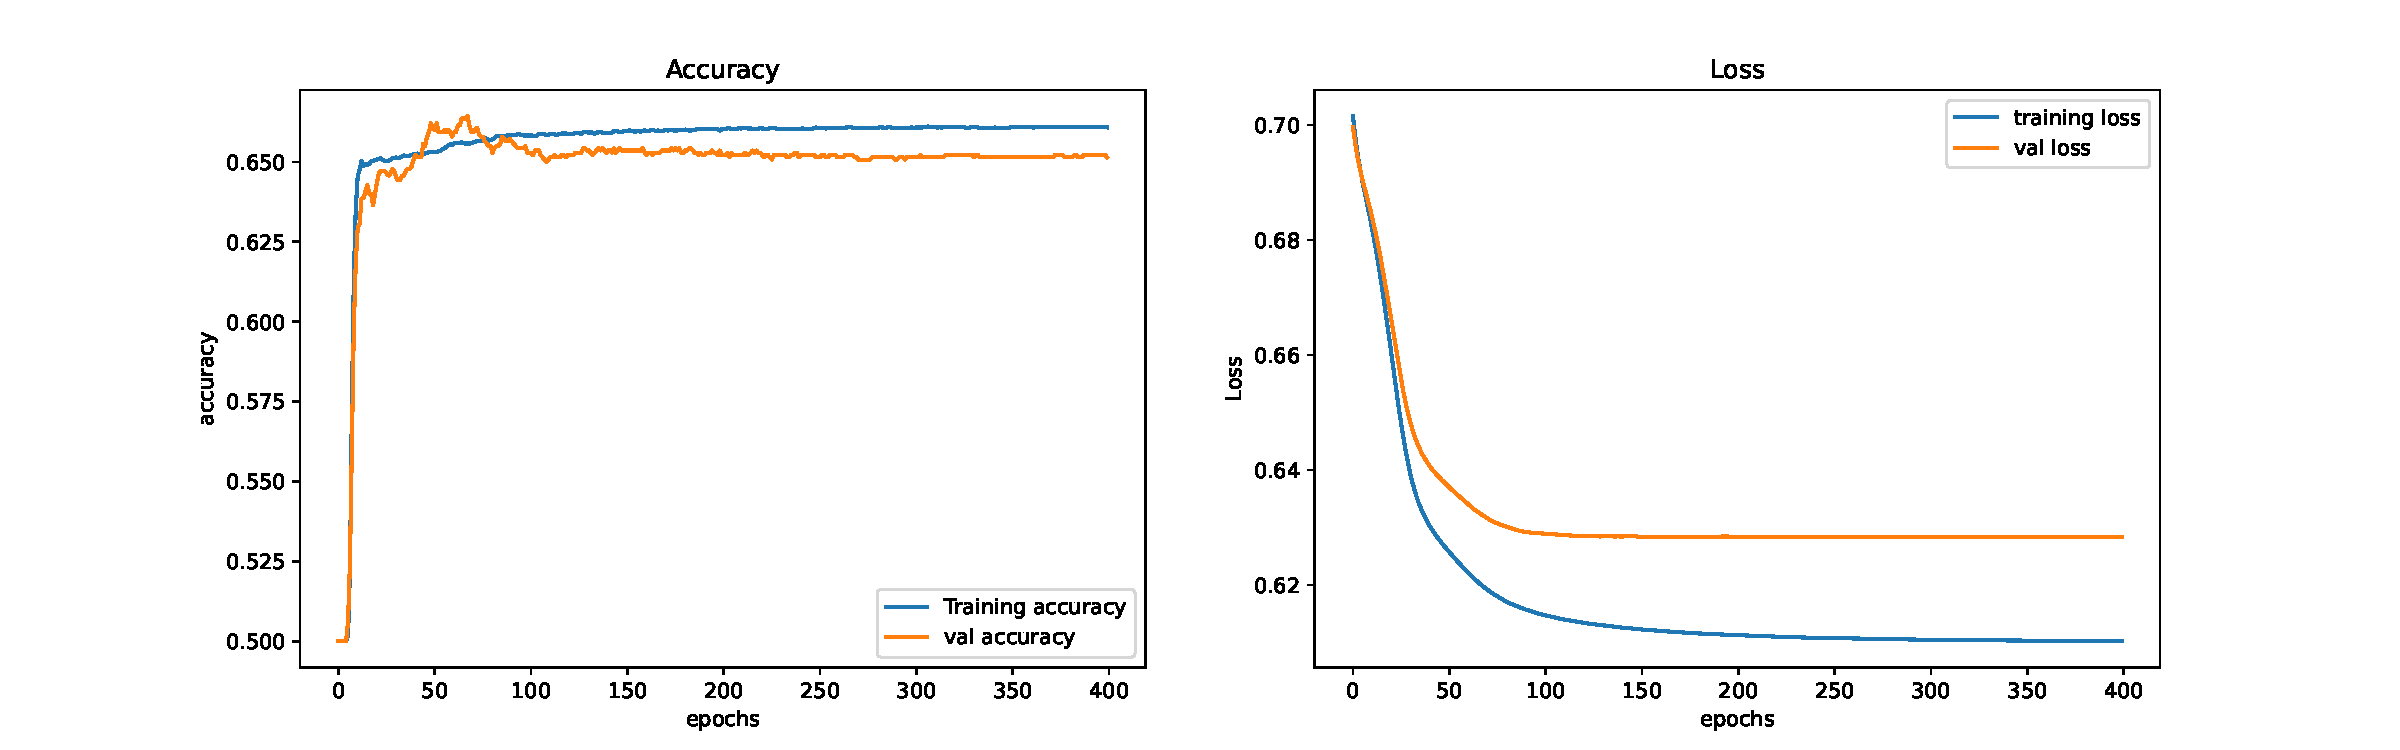
\includegraphics[width=\textwidth]{pictures/nn-history.pdf}
\caption{Learning history for dense neural network}
\label{nn-history}
\end{figure}
%

Here are the results (Table \ref{nn-result}).
%
\begin{table}[h]
\centering
\caption{Results of dense neural network}
\begin{tabular}{|l|c|c|c|c|}
\hline
& \textbf{nn\_result} & \textbf{nn\_certainty} & \textbf{nn\_profit\_PS}& \textbf{nn\_profit\_B365} \\
\hline
mean & $0.648571$ & $0.248283$ & $0.028236$ & $0.004179$ \\
\hline
std & $0.477587$ & $0.112056$ & $0.897069$ & $0.852810$ \\
\hline
min & $0.000000$ & $0.000079$ & $-1.000000$ & $-1.000000$ \\
\hline
25\% & $0.000000$ & $0.168713$ & $-1.000000$ & $-1.000000$ \\
\hline
median & $1.000000$ & $0.279645$ & $0.255000$ & $0.220000$ \\
\hline
75\% & $1.000000$ & $0.344565$ & $0.520000$ & $0.500000$ \\
\hline
max & $1.000000$ & $0.399053$ & $7.820000$ & $5.000000$ \\
\hline
\end{tabular}

\label{nn-result}
\end{table}
%

\subsection{Exploring alternative models \& important features}

To asses whether using a surface-specific data frame (``feature'') is the best strategy for predicting tennis matches, we created a second data frame that includes surface-specific variables as well as tournament-specific features, such as wins for each tournament on the ATP tour. To analyze the importance of the different variables in predicting our target variable ``PlayerA\_Wins'', we calculated the $20$ most important variables of the new data frame using the following standard machine learning models:
%
\begin{itemize}
\item Decision Tree (DT),
\item Random Forest (RF),
\item Ada Boost (AB),
\item Gradient Boosting (GB), and
\item Neural Network (NN).
\end{itemize}

\begin{figure}[h]
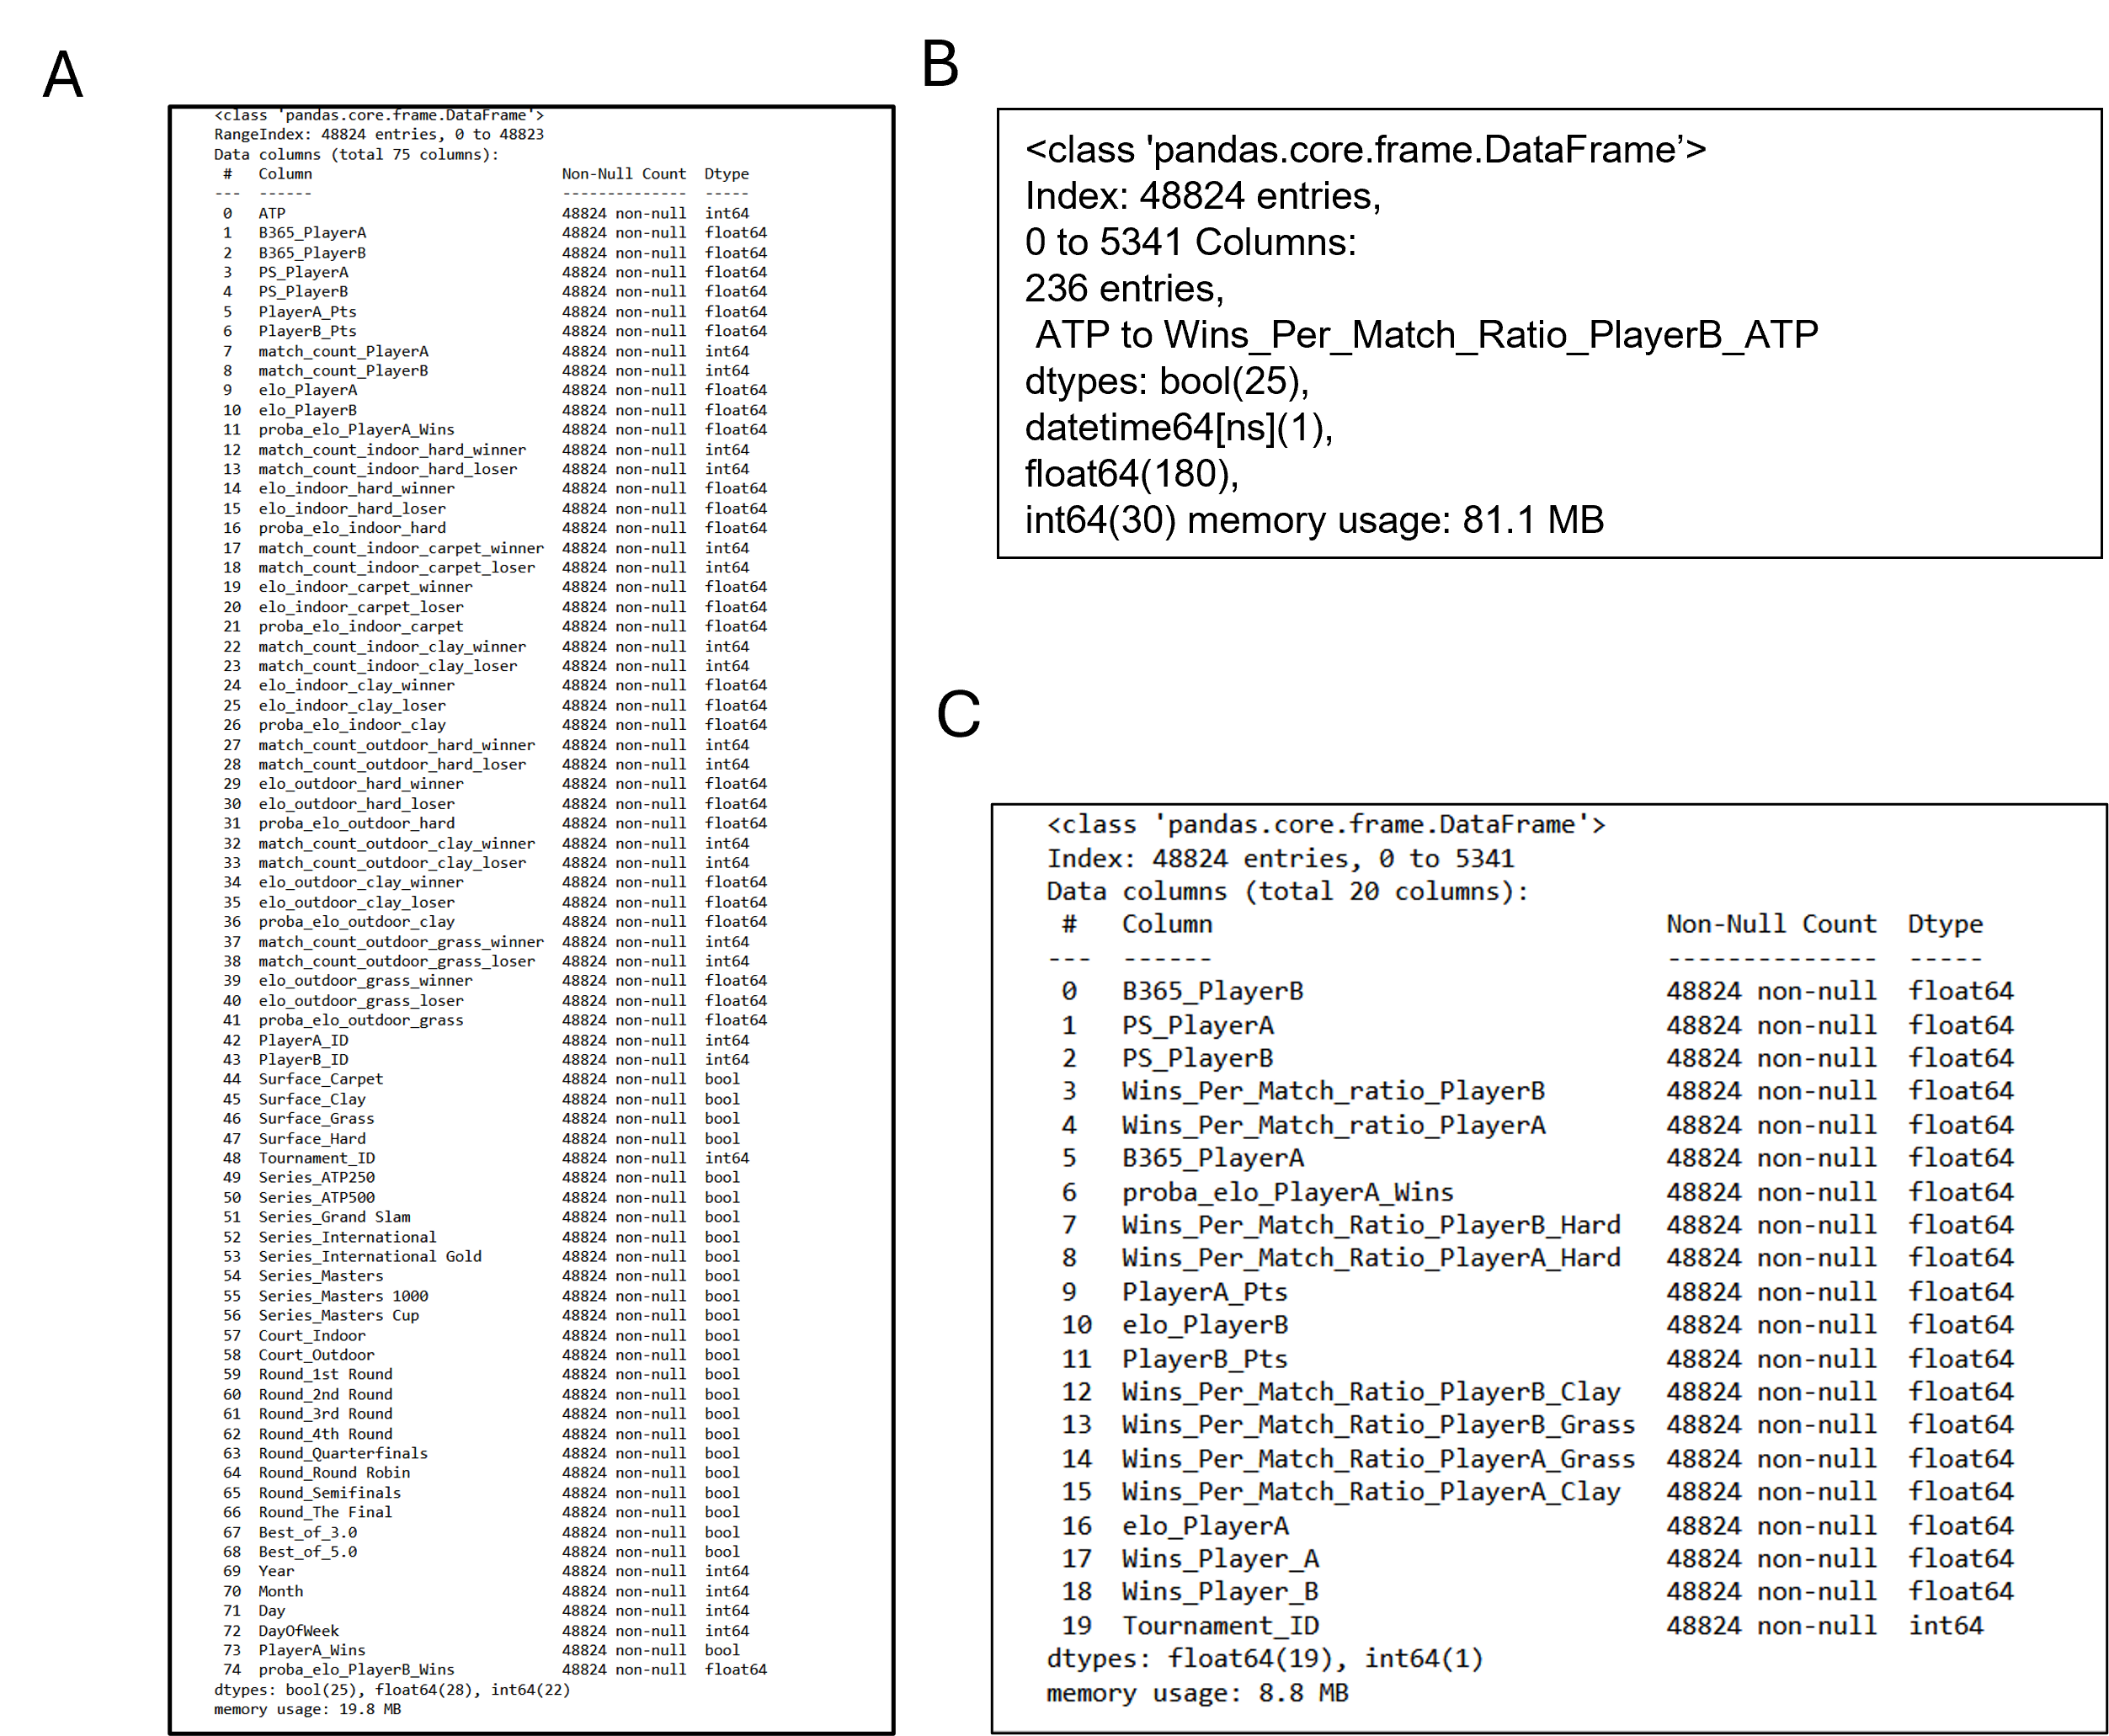
\includegraphics[width=\textwidth]{pictures/dataframes-patrick.png}
\caption{Data frames. A)  The Initial data frame. B) Engineered Data frame with 236 features, a detailed list of all the variables of this data frame can be found at additional data section of this document. C) Data frame containing top 20 features calculated from Random Forest model with the engineered data frame to predict.}
\label{dataframes-patrick}
\end{figure}
%

The images (Figure \ref{most-important-ada}, \ref{most-important-gb}, \ref{most-important-rf}, \ref{most-important-df}) indicate that all machine learning algorithms used share a common set of important features for predicting the target variable ``Player A wins''. Notably, across all features presented to the algorithms, the odds from Pinnacle Sports appear to be the most influential, followed by the individual win-per-match ratio (see Table \ref{top-10-features-table}). Additionally, the win-match ratio on the four different surfaces emerges as particularly significant in predicting the outcome of a tennis match.

%
\begin{figure}[h]
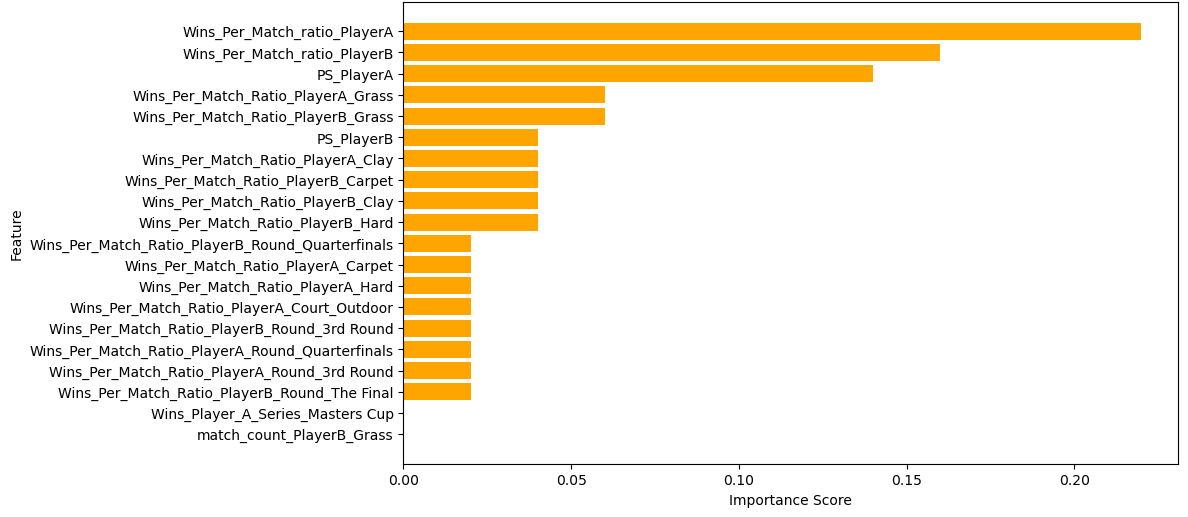
\includegraphics[width=\textwidth]{pictures/most-important-ada.png}
\caption{AdaBoost: Top 20 features predicting the target variable Player A wins.}
\label{most-important-ada}
\end{figure}
%
For AdaBoost the most important feature to predict the target variable are the wins per match ratio of each player.

%
\begin{figure}[h]
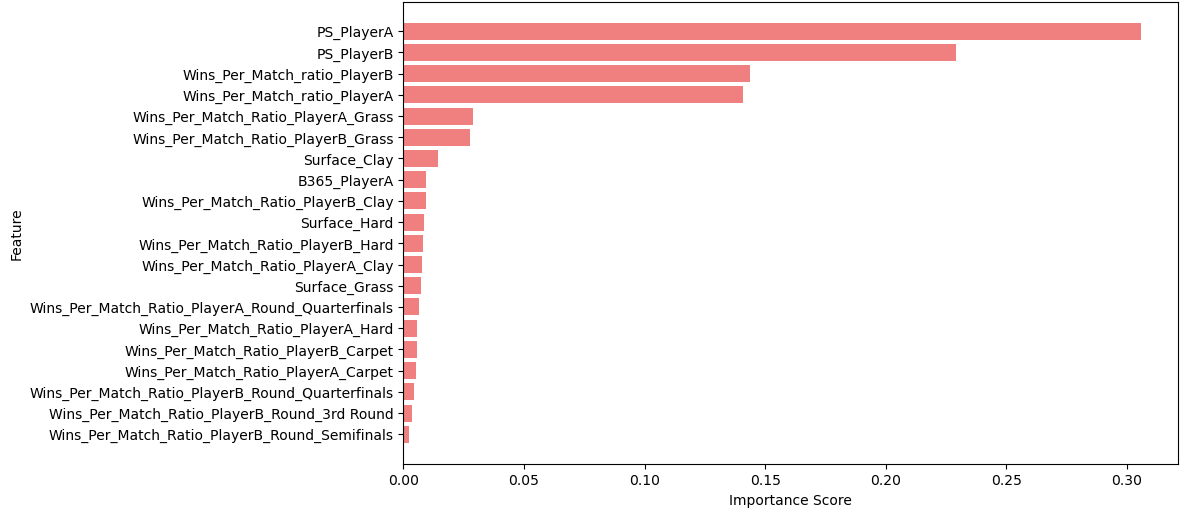
\includegraphics[width=\textwidth]{pictures/most-important-gb.png}
\caption{Gradient Boosting: Top 20 features predicting the target variable Player A wins.}
\label{most-important-gb}
\end{figure}
%
The odds of Pinnacle sports are of major importance to predict the outcome for the Gradient Boosting algorithm. 
%
\begin{figure}[h]
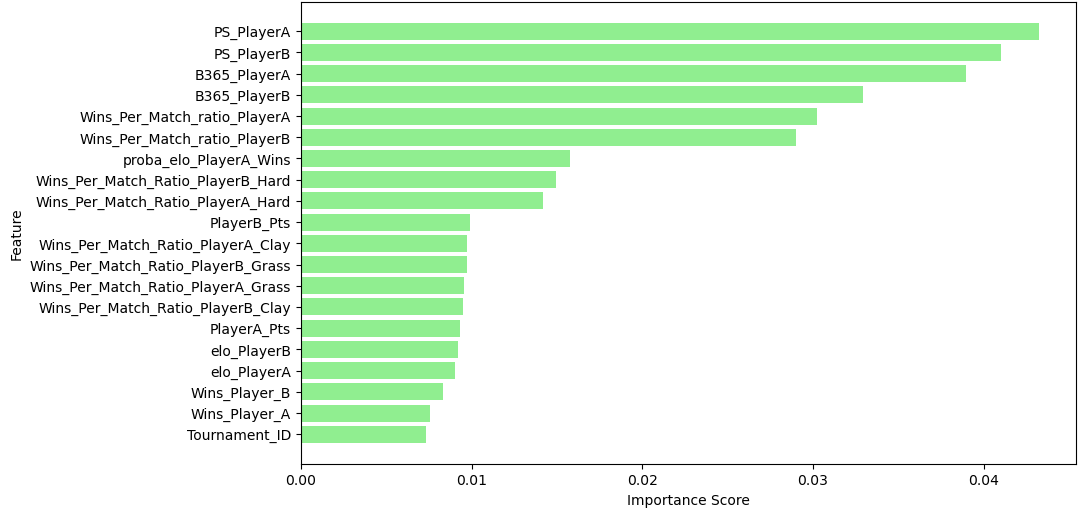
\includegraphics[width=\textwidth]{pictures/most-important-rf.png}
\caption{Random Forest: Top 20 features predicting the target variable Player A wins.}
\label{most-important-rf}
\end{figure}
%
Like the Gradient Bosting algorithm, the Random Forest algorithm highly relies on the odds of Pinnacle sports to predict the winner of the tennis match. 
%
\begin{figure}[h]
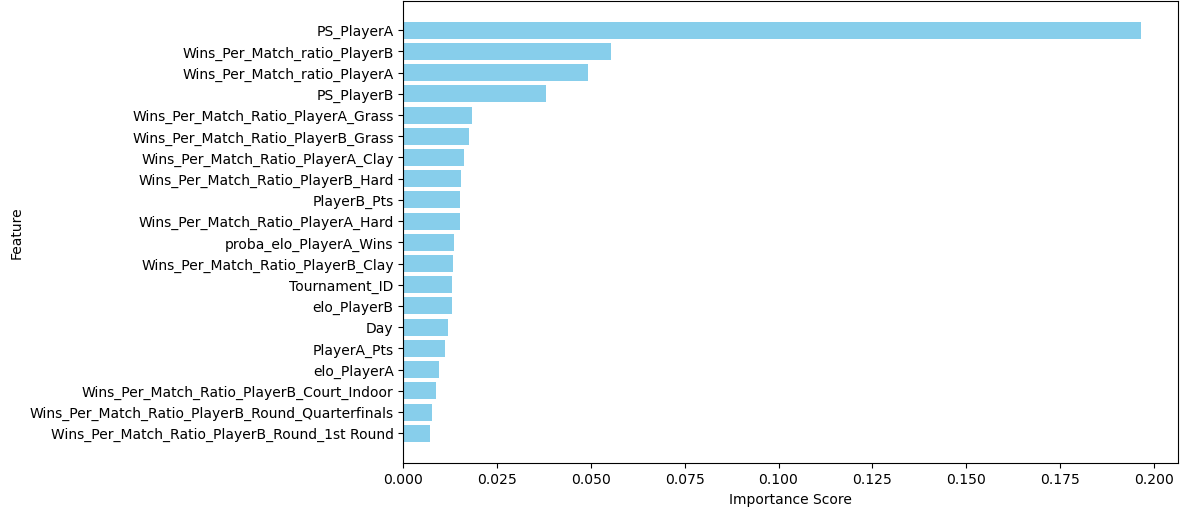
\includegraphics[width=\textwidth]{pictures/most-important-dt.png}
\caption{Decision Tree: Top 20 features predicting the target variable Player A wins.}
\label{most-important-df}
\end{figure}
%
The Decision Tree algorithm heavily relies on the odds from Pinnacle Sports, with the win-match ratios of Player A and Player B ranking second and fourth in importance, respectively.
In summary, it can be concluded that the odds from the bookmaker, along with the win-match ratios of each individual player on different surfaces, are the most critical features for predicting tennis match outcomes. Additionally, player points (word ranking system points), Elo ratings, and specific win-match ratios for particular tournaments also emerge as significant factors in predicting match outcomes.

\begin{table}[h]
\centering
\caption{Top 10 features predicting if Player A wins among DT,RF,AB, GB}
\begin{tabular}{|c|l|}
\hline
\textbf{Feature \#} & \textbf{Top 10 Features among all models} \\
\hline
1 & PS\_PlayerA \\
2 & Wins\_Per\_Match\_ratio\_PlayerB \\
3 & Wins\_Per\_Match\_ratio\_PlayerA \\
4 & PS\_PlayerB \\
5 & Wins\_Per\_Match\_Ratio\_PlayerA\_Grass \\
6 & Wins\_Per\_Match\_Ratio\_PlayerB\_Grass \\
7 & Wins\_Per\_Match\_Ratio\_PlayerA\_Clay \\
8 & Wins\_Per\_Match\_Ratio\_PlayerB\_Hard \\
9 & Wins\_Per\_Match\_Ratio\_PlayerA\_Hard \\
10 & Wins\_Per\_Match\_Ratio\_PlayerB\_Clay \\
\hline
\end{tabular}
\label{top-10-features-table}
\end{table}

The accuracy scores of all four standard ML algorithms, trained with their 20 most important features from the data frame, range between $65 \%$ (Decision Tree) and $76 \%$ (Gradient Boosting). In summary, it can be concluded that with Random Forest, AdaBoost, and Gradient Boosting, three out of four tennis matches can be correctly predicted (Figure \ref{accuracy-score-models}, \ref{confusion-matrix}).

%
\begin{figure}[h]
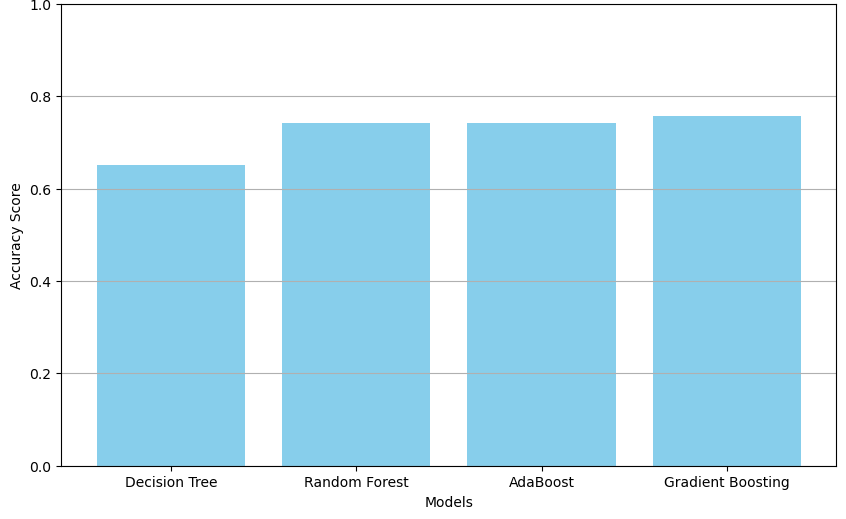
\includegraphics[width=\textwidth]{pictures/accuracy-score-models.png}
\caption{Accuracy scores of the Decision Tree, Random Forest, AdaBoost and Gradien Boosting for the Top 20 features data frame. Decision Tree: $0.65$, Random Forest: $0.74$, AdaBoost: $0.74$ and Gradient Boosting: $0.76$.}
\label{accuracy-score-models}
\end{figure}

To verify the calculated accuracy score for each model, we generated a confusion matrix for each (Figure \ref{confusion-matrix}). The data within the confusion matrices are consistent with the accuracy scores obtained. Approximately $75 \%$ of the matches are correctly predicted (either Player A wins or loses), while about $25 \%$ are wrongly predicted. There is no observable tendency indicating that the algorithm favors one outcome over the other.
%
\begin{figure}[h]
    \centering
    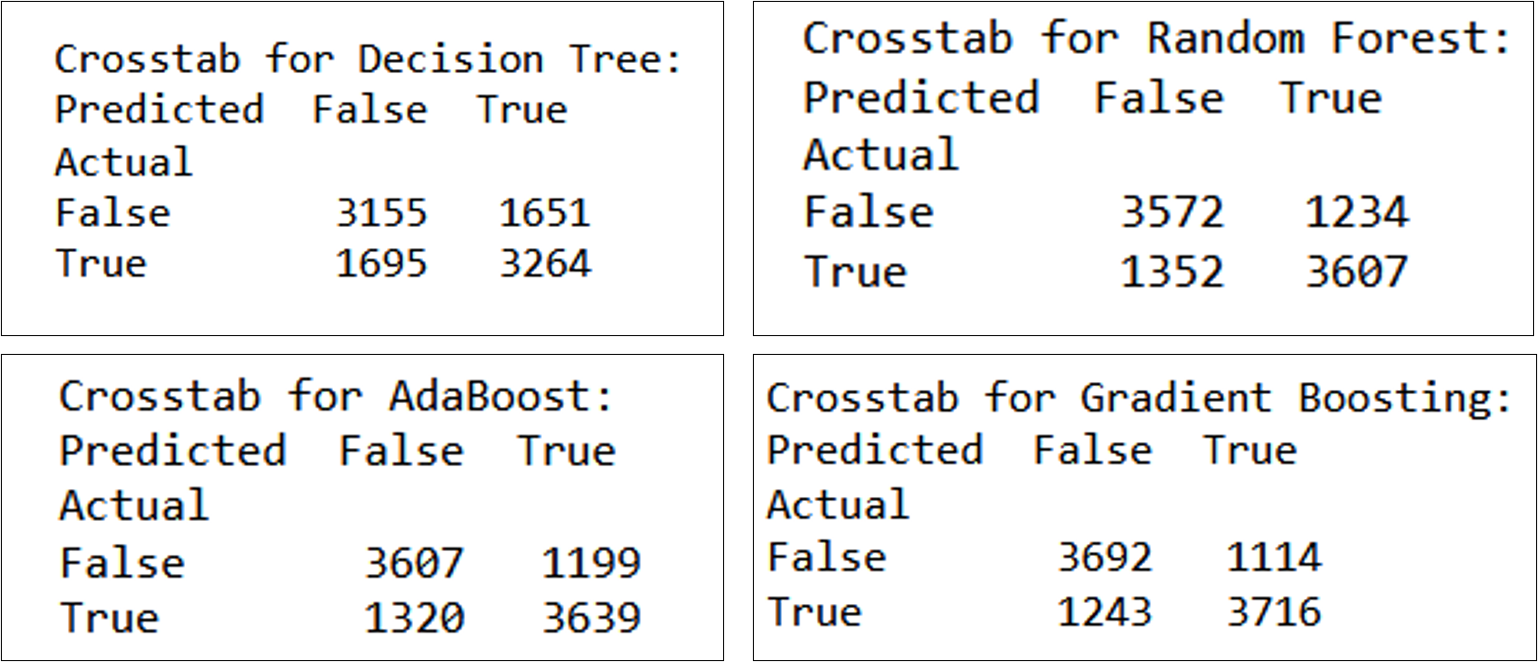
\includegraphics[width=\textwidth]{pictures/confusion-matrix.png}
    \caption{Confusion matrix of Decision Tree, Random Forest, AdaBoost and Gradient Boosting. The confusion matrix has been produced with the predicted values for each model compared to the $y\_test$ (Player A wins) set.}
    \label{confusion-matrix}
\end{figure}

%

%
\begin{figure}[h]
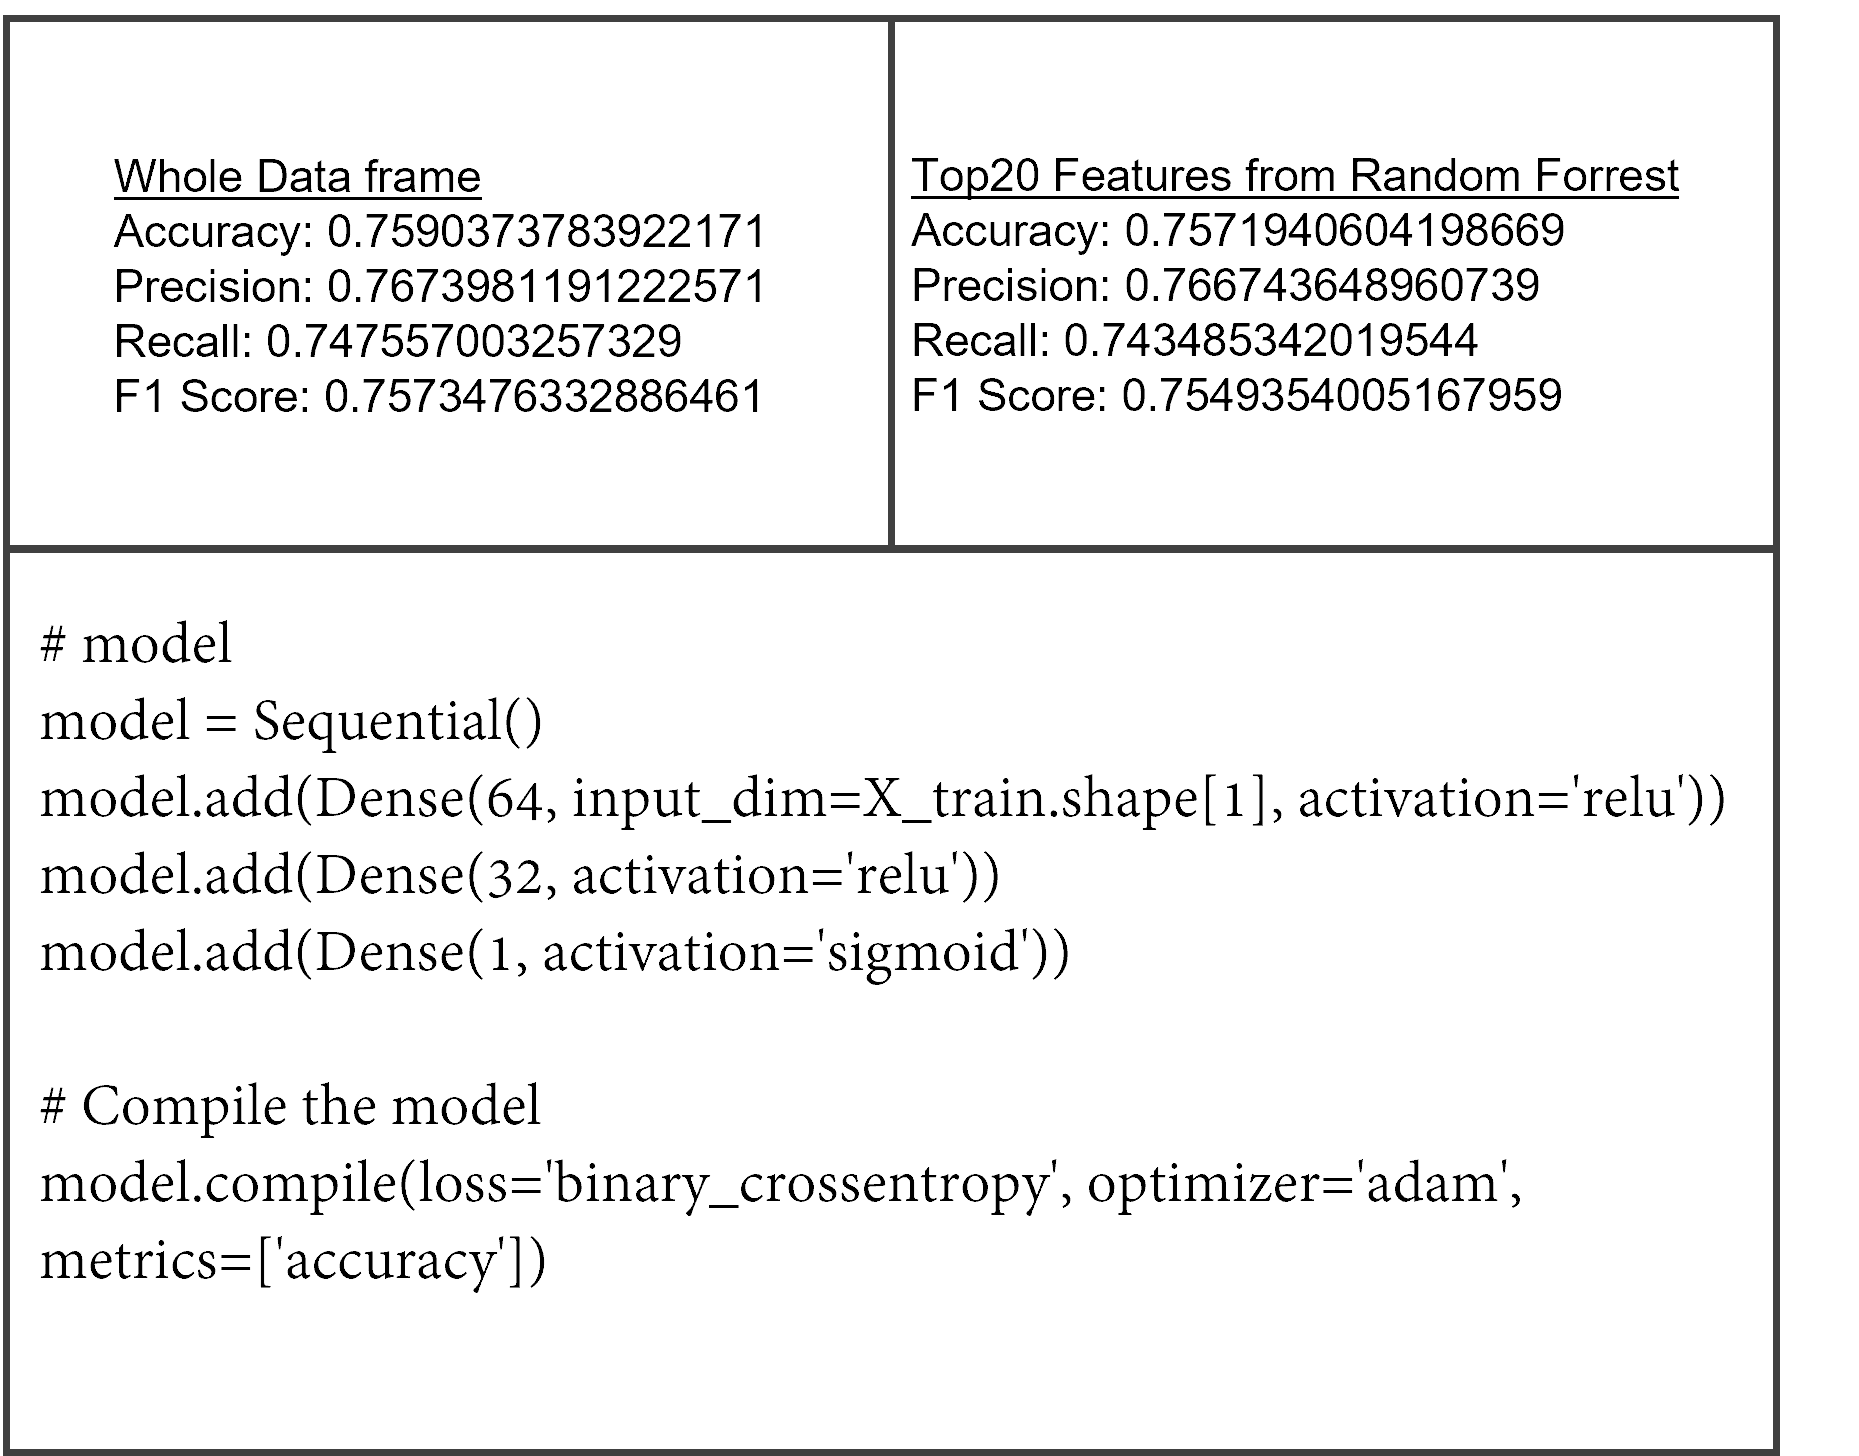
\includegraphics[width=\textwidth]{pictures/nn-model.png}
\caption{Prediction with Neural Network: A simple neural network has been trained with the Keras / Tensorflow library with the top 20 features from Random Forest to predict our target variable.}
\label{nn-moodel}
\end{figure}
%

%
\begin{figure}[h]
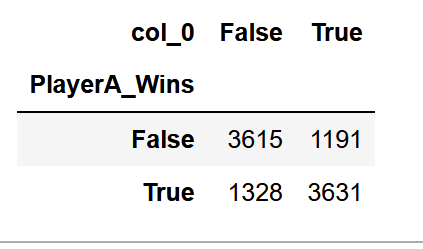
\includegraphics[width=\textwidth]{pictures/confusion-matrix-nn.png}
\caption{Confusion matrix of neural network prediction. The confusion matrix shows the predicted data plotted against the real data}
\label{confusion-matrix-nn}
\end{figure}
%

\subsection{Betting with the prediction model}

Our goal was not only to predict tennis matches but also to generate virtual profits with our predictions. We placed $1$ \$ on each predicted game and utilized the odds from Pinnacle Sports to calculate our return on investment (ROI). After betting on $9765$ tennis matches, we found that all our standard algorithms resulted in a negative ROI (Figure \ref{betting-strategy}). Despite our models correctly predicting $3$ out of $4$ tennis matches, we were unable to achieve a positive net amount of money after betting using the bookmaker's odds.
%
\begin{figure}[h]
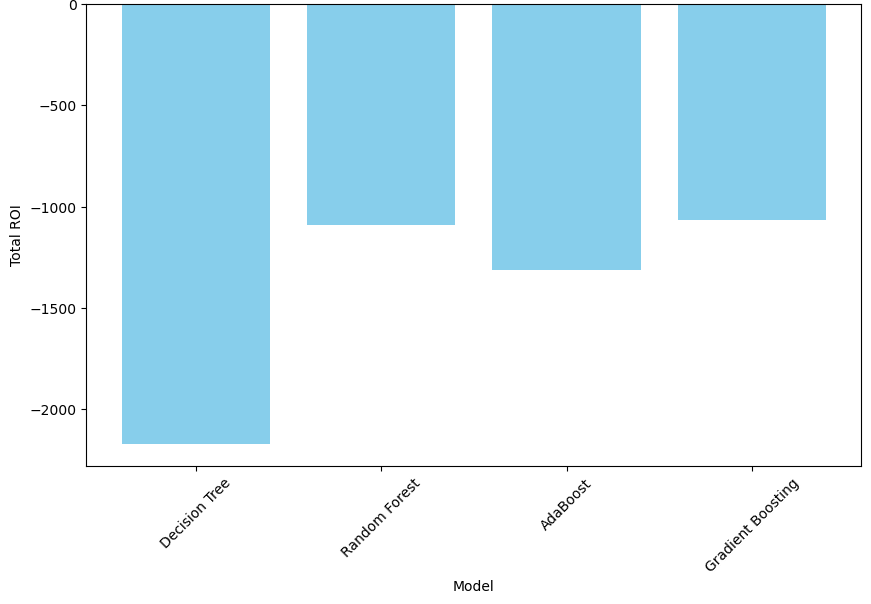
\includegraphics[width=\textwidth]{pictures/betting.png}
\caption{Return of investment after betting $1$ \$ on each predicted match by our algorithm.}
\label{betting-strategy}
\end{figure}
%

%\section{Post learning analysis \& packaging}
%
%
%\subsection{Uncertainty cutoff}
%
%
%\subsection{Cutoff optimization}


\section{Conclusion}

We were able to train five different models that can correctly predict three out of four tennis matches. Furthermore, we identified the most important features for correctly predicting the outcome of a tennis match. Unfortunately, the prediction accuracy of about $75 \%$ is not enough to generate a positive return on investment (ROI) using the odds from Pinnacle Sports. We also attempted to train our models on matches where both players have a high difference in Elo ratings, making it easier for the algorithm to correctly predict the winner (Data not shown). Although this strategy significantly improves the prediction accuracy, the odds on those games were so low that we wouldn’t achieve any positive ROI by betting on them. Since bookmakers' odds are designed to ensure a positive net income for the bookmaker in the long run, we should be cautious about including them in our model training. The odds set by bookmakers inherently favor the bookmaker and may negatively influence our prediction model. For future prediction models, we should not rely on bookmaker odds and instead focus more on the Elo system as well as calculated features such as a player's specific win ratio against an opponent. It might also be beneficial to aggregate important features into a single variable, such as the win ratio per match at a specific tournament and round. Another way to improve our models would be to utilize advanced neural networks like recurrent neural networks, especially Long Short-Term Memory (LSTM) networks, which incorporate time variables into their calculations and could enhance our prediction model.

%\begin{thebibliography}{9}
%\bibitem{Aksteiner:2016mol}
%S.~Aksteiner and T.~B\"ackdahl,
%``Symmetries of linearized gravity from adjoint operators,''
%J. Math. Phys. \textbf{60} (2019) no.8, 082501
%doi:10.1063/1.5092587
%[arXiv:1609.04584 [gr-qc]].
%\end{thebibliography}

%TOBE cited

\appendix

\begin{thebibliography}{9}
\bibitem{Silver:Mastering}
Silver, D., Schrittwieser, J., Simonyan, K. et al. Mastering the game of Go without human knowledge. Nature 550, 354–359 (2017). https://doi.org/10.1038/nature24270

\bibitem{Jumper:Highly}
Jumper, J., Evans, R., Pritzel, A. et al. Highly accurate protein structure prediction with AlphaFold. Nature 596, 583–589 (2021). https://doi.org/10.1038/s41586-021-03819-2

\bibitem{Turing:Computing}
A. M. Turing (1950) Computing Machinery and Intelligence. Mind 49: 433-460

\bibitem{Bulletin}
Bulletin of Mathematical Biology Vol. 52, No. l/2. pp. 99-115. 1990.

\bibitem{McCulloch:logical}
McCulloch, W.S., Pitts, W. A logical calculus of the ideas immanent in nervous activity. Bulletin of Mathematical Biophysics 5, 115–133 (1943). https://doi.org/10.1007/BF02478259

\bibitem{Applications}
Applications and Techniques for Fast Machine Learning in Science  
Frontiers in Big Data, VOLUME=5, YEAR=2022   
Iqbal H. Sarker
DOI=10.3389/fdata.2022.787421
Machine Learning: Algorithms, Real‑World Applications and Research
\end{thebibliography}

\end{document}